\newpage
\section{HỆ BẤT PHƯƠNG TRÌNH BẬC NHẤT HAI ẨN}
\subsection{LÝ THUYẾT CẦN NHỚ}
\subsubsection{HỆ BẤT PHƯƠNG TRÌNH BẬC NHẤT HAI ẨN}
\indam{\iconMT ~Định nghĩa:}
\begin{boxdn}
Hệ bất phương trình bậc nhất hai ẩn $x$, $y$ là một hệ gồm hai hay nhiều bất phương trình bậc nhất hai ẩn $x$, $y$. Mỗi nghiệm chung của các bất phương trình trong hệ được gọi là một nghiệm của hệ bất phương trình đó.
\end{boxdn}
	\begin{itemize}
		\item Cặp số $(x_0;y_0)$ là \textbf{nghiệm} của một hệ bất phương trình bậc nhất hai ẩn khi $(x_0;y_0)$ đồng thời là nghiệm của tất cả bất phương trình trong hệ đó.
		\item Miền nghiệm của hệ bất phương trình là giao các miền nghiệm của các bất phương trình trong hệ.
	\end{itemize}
\subsubsection{BIỂU DIỄN MIỀN NGHIỆM CỦA HỆ BẤT PHƯƠNG TRÌNH BẬC NHẤT HAI ẨN TRÊN MẶT PHẲNG TỌA ĐỘ}
\begin{enumerate}[\iconMT]
	\item \indam{Định nghĩa:} 
		\begin{boxdn} Miền nghiệm của hệ bất phương trình là giao các miền nghiệm của các bất phương trình trong hệ.
	\end{boxdn}
	\item \indam{Cách xác định miền nghiệm của một hệ bất phương trình bậc nhất hai ẩn:}
	 Để biểu diễn miền nghiệm của hệ bất phương trình bậc nhất hai ẩn, ta làm như sau:
		\begin{itemize}
			\item Trong cùng mặt phẳng tọa độ, biểu diễn miền nghiệm của mỗi bất phương trình trong hệ bằng cách gạch bỏ phần không thuộc miền nghiệm của nó.
			\item Phần không bị gạch là miền nghiệm cần tìm.
		\end{itemize}
\end{enumerate}
\subsubsection{ỨNG DỤNG CỦA HỆ BẤT PHƯƠNG TRÌNH BẬC NHẤT HAI ẨN}
Để tìm giá trị lớn nhất, giá trị nhỏ nhất của biểu thức dạng $F = ax + by$, trong đó $x$, $y$ là nghiệm của một hệ bất phương trình bậc nhất hai ẩn $x$, $y$ mà miền nghiệm của hệ đó là một miền đa giác, ta làm như sau:
\begin{itemize}
	\item Bước 1: Xác định miền nghiệm của hệ bất phương trình (là một miền đa giác).
	\item Bước 2: Xác định tọa độ các đỉnh của đa giác.
	\item Bước 3: Tính giá trị của biểu thức $F = ax + by$ tại cặp số $(x; y)$ là tọa độ các đỉnh của đa giác rồi so sánh các giá trị đó. Từ đó, kết luận được giá trị lớn nhất hay giá trị nhỏ nhất cần tìm.
\end{itemize}
%-------------------------------------------------------------------------------------------------------------
\subsection{PHÂN LOẠI VÀ PHƯƠNG PHÁP GIẢI TOÁN}
\begin{dang}{Nhận dạng hệ bất phương trình bậc nhất hai ẩn}
	Dựa vào định nghĩa để nhận dạng hệ bất phương trình bậc nhất hai ẩn: Hệ bất phương trình bậc nhất hai ẩn $x$, $y$ là một hệ gồm hai hay nhiều bất phương trình bậc nhất hai ẩn $x$, $y$.
\end{dang}
\begin{vd}%[Dự án đề cương 3 khối NH24-25 Đợt 1-Nguyễn Tiến Liên]%[0D2N2-1]
	Hệ bất phương trình nào sau đây là hệ bất phương trình bậc nhất hai ẩn? 
	\choice 
	{$\heva{&- 8 x - 3 y^2 + 8 \ge 0 \\ &- x - 2y - 9 \le 0}$}
	{\True $\heva{&- 6x+y - 6 \le 0 \\ &9x - 2 \le 0}$}
	{$\heva{&- 3x^2 - 9y - 4 > 0 \\ &3x + 7y \ge 0}$}
	{$\heva{&- 2x^2 + 4y^2 + 4 < 0 \\ &- 2x + y - 2 > 0}$}

	\loigiai{Hệ bất phương trình $\heva{&- 6x+y - 6 \le 0 \\ &9x - 2 \le 0}$ là hệ bất phương trình bậc nhất hai ẩn.}
\end{vd}
\begin{vd}%[Dự án đề cương 3 khối NH24-25 Đợt 1-Nguyễn Tiến Liên]%[0D2N2-1]
	Hệ bất phương trình nào sau đây là hệ bất phương trình bậc nhất hai ẩn? 
	\choice 
	{$\heva{&- 3x - 17 y^2 + 4 > 0 \\ &x - 4y - 9 > 0}$}
	{$\heva{&5 x^2 + 6 y - 9 > 0 \\ &- 6x - 4y + 4 \le 0}$}
	{$\heva{&- 5x^2 + 3 y^{2} - 3 \ge 0 \\ &6x - 6y - 5 < 0}$}
	{\True $\heva{&- 8x - y + 3 > 0 \\ &6 x + 9y - 4 \ge 0}$}
	\loigiai{Hệ bất phương trình $\heva{&- 8x - y + 3 > 0 \\ &6 x + 9 y - 4 \ge 0}$ là hệ bất phương trình bậc nhất hai ẩn.}
\end{vd}
\begin{dang}{Kiểm tra cặp số $(x_0;y_0)$ là nghiệm  của hệ bất phương trình bậc nhất hai ẩn}
Cặp số $(x_0;y_0)$ là \textbf{nghiệm} của một hệ bất phương trình bậc nhất hai ẩn khi $(x_0;y_0)$ đồng thời là nghiệm của tất cả bất phương trình trong hệ đó.
\end{dang}
\begin{vd}%[Dự án đề cương 3 khối NH24-25 Đợt 1-Nguyễn Tiến Liên]%[0D2N2-2]
Cho hệ bất phương trình bậc nhất hai ẩn $\heva{& - 5 x - y + 3 > 0 \\ & 5 x - 2 y - 2 < 0}$. Cặp số nào dưới đây là một nghiệm của hệ? 
\choice 
{\True $(-1;1)$}
{$(8;1)$}
{$(1;7)$}
{$(1;4)$}
\loigiai{Cặp số $(-1;1)$ thỏa mãn cả hai bất phương trình của hệ nên nó là một nghiệm của hệ bất phương trình bậc nhất hai ẩn đã cho.}
\end{vd}
\begin{vd}%[Dự án đề cương 3 khối NH24-25 Đợt 1-Nguyễn Tiến Liên]%[0D2N2-2]
Miền nghiệm của hệ bất phương trình $\heva{& -x-2y<3\\& 3x-y<0\\& x+8y>1}$ chứa điểm nào sau đây? 
\choice 
{$(1;-4)$}
{$(-5;-3)$}
{\True $(-5;4)$}
{$(8;3)$}
\loigiai{Cặp số $(-5;4)$ thỏa mãn tất cả các bất phương trình trong hệ nên thuộc miền nghiệm của hệ đã cho.}
\end{vd}
\begin{dang}{Biểu diễn miền nghiệm của một hệ bất phương trình bậc nhất hai ẩn}
	\begin{enumerate}[\bf B1.]
		\item  Trong cùng mặt phẳng tọa độ, biểu diễn miền nghiệm của mỗi bất phương trình trong hệ bằng cách gạch bỏ phần không thuộc miền nghiệm của nó.
		\item   Phần không bị gạch là miền nghiệm cần tìm.
	\end{enumerate}
\end{dang}
\begin{vd}%[Dự án đề cương 3 khối NH24-25 Đợt 1-Nguyễn Tiến Liên]%[0D2H2-2]
Biểu diễn miền nghiệm của hệ bất phương trình $\heva{& x+y \le -4 \\& x-y \ge -2.}$
	\loigiai{
		\immini{Vẽ các đường thẳng $d_1\colon x+y=-4$ và $d_2\colon x-y=-2$.\\
		Gạch đi các phần không thuộc miền nghiệm của mỗi bất phương trình.\\
		Miền nghiệm của hệ bất phương trình là phần không bị gạch kể cả hai tia $Ad_1$ và $Ad_2$ với $A(-3;-1)$.}
	{
		\begin{tikzpicture}[scale=0.75, font=\footnotesize, line join=round, line cap=round, >=stealth]
			\def\xmin{-5}
			\def\xmax{3}
			\def\ymin{-3}
			\def\ymax{5}
			\path
			(0,\ymax) coordinate (y)
			(0,0) coordinate (O)
			(\xmax,0) coordinate (x);
			\draw[->] (\xmin,0)--(\xmax,0)node[right]{$x$};
			\draw[->] (0,\ymin)--(0,\ymax)node[above]{$y$};
			\fill (0,0) circle (1pt) node[below left]{O};
			\draw pic[draw,angle radius=1mm] {right angle = y--O--x};
			\clip (\xmin,\ymin) rectangle (\xmax,\ymax);
			\draw[samples=150,domain=\xmin:\xmax]plot(\x,{-4-(\x)});
			\draw[samples=150,domain=\xmin:\xmax]plot(\x,{2+(\x)});
			\path
			(-3,-1) coordinate (A)
			;
			\foreach \x/\g in {A/180} \fill[black] (\x) circle (1pt)+(\g:.3) node {$\x$};
			%			\fill[opacity=0.2,pattern=north west lines](\xmin,\ymin)--(\xmin,\ymax)-- (0,\ymax)--(0,\ymin)--cycle;
			\fill[opacity=0.4,pattern=north west lines](\xmin,\ymax)--plot[domain=\xmin:\xmax] (\x,{-4-\x})--(\xmax,\ymin)--(\xmax,\ymax)--cycle;
			\fill[opacity=0.3, blue](\xmin,\ymax)--plot[domain=\xmin:\xmax] (\x,{2+(\x)})--(\xmax,\ymin)--(\xmax,\ymax)--cycle;
			%			\fill[opacity=0.2,green](\xmin,\ymin)--(\xmin,0)-- (\xmax,0)--(\xmax,\ymin)--cycle;
			\node at (-1.2,\ymin)[above left]{$d_1$};
			\node at (\xmin+0.3,\ymin)[above right]{$d_2$};
			\end{tikzpicture}
		}
			}
\end{vd}
\begin{vd}%[Dự án đề cương 3 khối NH24-25 Đợt 1-Nguyễn Tiến Liên]%[0D2H2-2]
	Biểu diễn hình học tập nghiệm của hệ bất phương trình
	$ \heva{& 3x + y \le 6 \\& x + y \le 4 \\& x \ge 0 \\& y \ge 0. } $
	\loigiai{
	\immini{
	Vẽ các đường thẳng $d_1 \colon 3x + y = 6$; $d_2 \colon x + y = 4$; $d_3 \colon x = 0$ (trục $Oy$);\\
	 $d_4 \colon y = 0$ (trục $Ox$).\\
	Vì điểm $M_0(1;1)$ có tọa độ thỏa mãn tất cả các bất phương trình trong hệ trên nên ta tô màu các nửa mặt phẳng bờ $d_1$, $d_2$, $d_3$, $d_4$ không chứa điểm $M_0$.\\
	Miền không bị tô màu (hình tứ giác $OCIA$ kể cả bốn cạnh $AI$, $IC$, $CO$, $OA$ ) trong hình vẽ là miền nghiệm của hệ đã cho.}{
			\begin{tikzpicture}[scale=1, font=\footnotesize, line join=round, line cap=round, >=stealth]
				\def\xmin{-1}
				\def\xmax{5}
				\def\ymin{-1}
				\def\ymax{7}
				\path
				(0,\ymax) coordinate (y)
				(0,0) coordinate (O)
				(\xmax,0) coordinate (x);
				\draw[->] (\xmin,0)--(\xmax,0)node[right]{$x$};
				\draw[->] (0,\ymin)--(0,\ymax)node[above]{$y$};
				\fill (0,0) circle (1pt) node[below left]{O};
				\draw pic[draw,angle radius=1mm] {right angle = y--O--x};
				\clip (\xmin,\ymin) rectangle (\xmax,\ymax);
				\draw[samples=150,domain=\xmin:\xmax]plot(\x,{6-3*(\x)});
				\draw[samples=150,domain=\xmin:\xmax]plot(\x,{4-(\x)});
				\path
				(0,4) coordinate (A)
				(0,6) coordinate (B)
				(2,0) coordinate (C)
				(4,0) coordinate (D)
				(1,3) coordinate (I);
				\foreach \x/\g in {A/180,B/180,C/-120,D/-90,I/40} \fill[black] (\x) circle (1pt)+(\g:.3) node {$\x$};
				\fill[opacity=0.4,pattern=north west lines](\xmin,\ymin)--(\xmin,\ymax)-- (0,\ymax)--(0,\ymin)--cycle;
				\fill[opacity=0.2,red](\xmin,\ymax)--plot[domain=\xmin:\xmax] (\x,{4-\x})--(\xmax,\ymin)--(\xmax,\ymax)--cycle;
				\fill[opacity=0.2, blue](-1/3,7)--plot[domain=-1/3:7/3] (\x,{6-3*(\x)})--(\xmax,\ymin)--(\xmax,\ymax)--cycle;
				\fill[opacity=0.2,green](\xmin,\ymin)--(\xmin,0)-- (\xmax,0)--(\xmax,\ymin)--cycle;
				\node at (7/3,-0.75)[right]{$d_1$};
				\node at (\xmax-0.3,-0.5)[below left]{$d_2$};
			\end{tikzpicture}}
	}
\end{vd}
\begin{dang}{Tìm giá trị lớn nhất, nhỏ nhất của biểu thức $T(x,y)=ax+by$ với $(x;y)$ nghiệm đúng một hệ bất phương trình bậc nhất hai ẩn cho trước}
		Để tìm giá trị lớn nhất, giá trị nhỏ nhất của biểu thức dạng $F = ax + by$, trong đó $x$, $y$ là nghiệm của một hệ bất phương trình bậc nhất hai ẩn $x$, $y$ mà miền nghiệm của hệ đó là một miền đa giác, ta làm như sau:
		\begin{enumerate}[\bf B1.]
		\item Xác định miền nghiệm của hệ bất phương trình đã cho. Kết quả thường được miền nghiệm $S$ là đa giác.
		\item Tính giá trị của $F$ tương ứng với $(x;y)$ là tọa độ của các đỉnh của đa giác.
		\item Kết luận\begin{itemize}
			\item Giá trị lớn nhất của $F$ là số lớn nhất trong các giá trị tìm được.
			\item Giá trị nhỏ nhất của $F$ là số nhỏ nhất trong các giá trị tìm được.
		\end{itemize}
	\end{enumerate}
\end{dang}
\begin{vd}%[Dự án đề cương 3 khối NH24-25 Đợt 1-Nguyễn Tiến Liên]%[0D2V2-2]
	Tìm giá trị lớn nhất, giá trị nhỏ nhất của
	\begin{enumerate}
		\item $T=2x+y$ với $(x;y)$ là nghiệm của hệ bất phương trình $\heva{&x-y-3\le 0\\&x\ge0\\&x+3y-3\le 0.}$
		\item $F=30x-4y-6$ với $(x;y)$ là nghiệm của hệ bất phương trình $\heva{&x-y+5\ge 0\\&2x+y+4\ge0\\&x+y-5\le 0\\&2x-y-4\le 0.}$
	\end{enumerate}
	\loigiai{
		\begin{enumerate}
			\item
			\immini{Miền nghiệm của hệ bất phương trình $\heva{&x-y-3\le 0\\&x\ge0\\&x+3y-3\le 0}$ là miền tam giác $ABC$ kể cả bờ, với $A(3;0)$, $B(0;1)$, $C(0;-3)$.\\
				$T(3;0)=6$, $T(0;1)=1$, $T(0;-3)=-3$.\\
				Vậy giá trị lớn nhất là $T=6$ và giá trị nhỏ nhất là $T=-3$.}
			{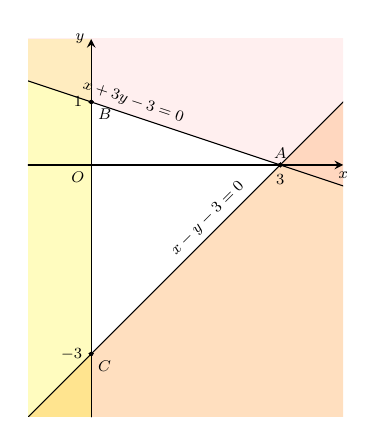
\begin{tikzpicture}[scale=0.8,font=\footnotesize,line join=round,line cap=round,>=stealth]
					\tikzset{every node/.style={scale=0.7}}
					\begin{scope}
						\clip (-1,-4) rectangle (4,2);
						\fill[orange,opacity=0.25] (-2,-5)--(6,-5)--(6,3)--cycle;
						\fill[yellow,opacity=0.25] (0,-4)--(-1,-4)--(-1,2)--(0,2)--cycle;
						\fill[pink,opacity=0.25] (-4,2.33)--(16,2.33)--(16,-4.33)--cycle;
						\fill (0,1) circle (1pt) node[below right]{$B$};
						\fill (3,0) circle (1pt) node[above]{$A$};
						\fill (0,-3) circle (1pt) node[below right]{$C$};
						\draw (5,2)--(-1,-4) node [pos=0.5, above, sloped] {$x-y-3=0$};
						\draw (-3,2)--(15,-4) node [pos=0.2, above, sloped] {$x+3y-3=0$};
					\end{scope}
					\draw[->] (-1,0)--(4,0) node[below]{$x$};
					\draw[->] (0,-4)--(0,2) node[left]{$y$};
					\draw (0,0) node[below left]{$O$};
					\foreach \x in {3}
					\draw[thin] (\x,1pt)--(\x,-1pt) node [below] {$\x$};
					\foreach \y in {-3,1}
					\draw[thin] (1pt,\y)--(-1pt,\y) node [left] {$\y$};
			\end{tikzpicture}}
			\item
			\immini{Miền nghiệm của hệ bất phương trình $\heva{&x-y+5\ge 0\\&2x+y+4\ge0\\&x+y-5\le 0\\&2x-y-4\le 0}$ là miền tứ giác $ABCD$ kể cả bờ, với $A(-3;2)$, $B(0;-4)$, $C(3;2)$, $D(0;5)$.\\
				$F(-3;2)=-104$, $F(0;-4)=10$, $F(3;2)=66$ và $F(0;5)=-26$.\\
				Vậy giá trị lớn nhất là $F=66$ và giá trị nhỏ nhất là $F=-104$.}
			{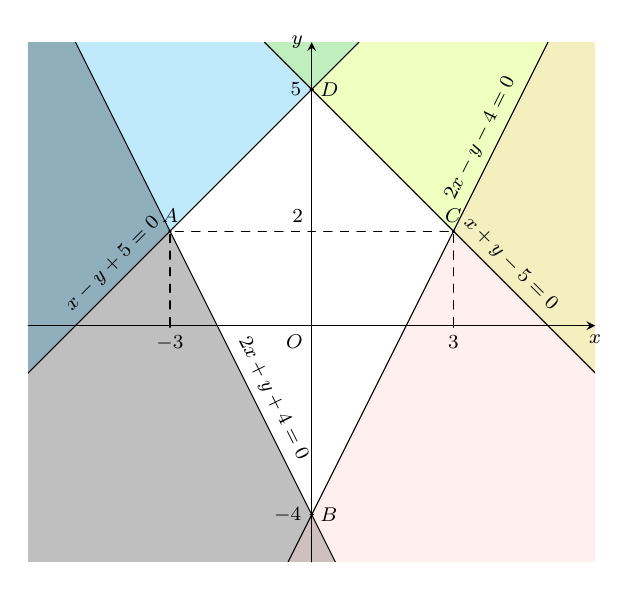
\begin{tikzpicture}[scale=0.6,font=\footnotesize,line join=round,line cap=round,>=stealth]
					\tikzset{every node/.style={scale=0.9}}
					\begin{scope}
						\clip (-6,-5) rectangle (6,6);
						\fill[cyan,opacity=0.25] (-11,-6)--(-11,12)--(7,12)--cycle;
						\fill[black,opacity=0.25] (-7,10)--(-7,-18)--(7,-18)--cycle;
						\fill[lime,opacity=0.25] (-7,12)--(11,12)--(11,-6)--cycle;
						\fill[pink,opacity=0.25] (-7,-18)--(7,-18)--(7,10)--cycle;
						\fill (-3,2) circle (1pt) node[above]{$A$};
						\fill (0,5) circle (1pt) node[right]{$D$};
						\fill (3,2) circle (1pt) node[above]{$C$};
						\fill (0,-4) circle (1pt) node[right]{$B$};
						\draw (1,6)--(-10,-5) node [pos=0.45, above, sloped] {$x-y+5=0$};
						\draw (-5,6)--(0.5,-5) node [pos=0.7, above, sloped] {$2x+y+4=0$};
						\draw (-1,6)--(10,-5) node [pos=0.45, above, sloped] {$x+y-5=0$};
						\draw (5,6)--(-0.5,-5) node [pos=0.2, above, sloped] {$2x-y-4=0$};
					\end{scope}
					\draw[->] (-6,0)--(6,0) node[below]{$x$};
					\draw[->] (0,-5)--(0,6) node[left]{$y$};
					\draw (0,0) node[below left]{$O$};
					\foreach \x in {-3,3}
					\draw[thin] (\x,1pt)--(\x,-1pt) node [below] {$\x$};
					\foreach \y in {-4,5}
					\draw[thin] (1pt,\y)--(-1pt,\y) node [left] {$\y$};
					\draw(0,2)node[above left]{$2$};
					\draw[dashed,thin] (-3,0)--(-3,2)--(0,2);
					\draw[dashed,thin] (3,0)--(3,2)--(0,2);
			\end{tikzpicture}}
		\end{enumerate}
	}
\end{vd}
%%VD2.2
\begin{vd}%[Dự án đề cương 3 khối NH24-25 Đợt 1-Nguyễn Tiến Liên]%[0D2V2-2]
	Tìm trị lớn nhất của biểu thức
	\begin{enumerate}
		\item $F(x;y)=x+2y$ với điều kiện $\heva{&0\le y\le 4\\&x\ge 0\\&x-y-1\le 0\\&x+2y-10\le 0.}$
		\item $F(x;y)=2x-3y$ với điều kiện $\heva{&y\le 0\\&x\ge 0\\&x+y-3\le 0\\&x+2y-4\le 0.}$
	\end{enumerate}
	\loigiai{
		\begin{enumerate}
			\item	\immini{\begin{itemize}
					\item Vẽ đường thẳng $d_1\colon x-y-1=0$, đường thẳng $d_1$ đi qua hai điểm $(0;-1)$ và $(1;0)$.
					\item Vẽ đường thẳng $d_2\colon x+2y-10=0$, đường thẳng $d_2$ đi qua hai điểm $(0;5)$ và $(2;4)$.
					\item Vẽ đường thẳng $d_3\colon y=4$.
				\end{itemize}
				Từ đó ta có miền nghiệm là miền ngũ giác $AOBCD$ với $A(0;4)$, $B(1;0)$, $C(4;3)$, $D(2;4)$ kể cả các cạnh.\\
				Ta có $F(4;3)=10$, $F(2;4)=10$, $F(0;4)=8$, $F(1;0)=1$ và $F(0;0)=0$.\\
				Vậy giá trị lớn nhất của biểu thức $F(x;y)=x+2y$ bằng $10$.}
			{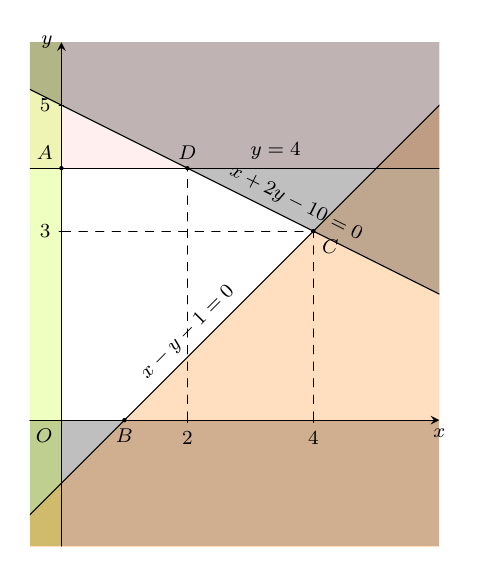
\begin{tikzpicture}[scale=0.8,font=\footnotesize,line join=round,line cap=round,>=stealth]
					\tikzset{every node/.style={scale=0.9}}
					\begin{scope}
						\clip (-0.5,-2) rectangle (6,6);
						\fill[black,opacity=0.25] (-0.5,0)--(-0.5,-2)--(6,-2)--(6,0)--cycle;
						\fill[pink,opacity=0.25] (-0.5,4)--(-0.5,6)--(6,6)--(6,4)--cycle;
						\fill[lime,opacity=0.25] (0,-2)--(-0.5,-2)--(-0.5,6)--(0,6)--cycle;
						\fill[orange,opacity=0.25] (-1.5,-2.5)--(8,-2.5)--(8,7)--cycle;
						\fill[black,opacity=0.25] (-2.5,6.25)--(15,6.25)--(15,-2.5)--cycle;
						\fill (2,4) circle (1pt) node[above]{$D$};
						\fill (0,4) circle (1pt) node[above left]{$A$};
						\fill (4,3) circle (1pt) node[below right]{$C$};
						\fill (1,0) circle (1pt) node[below]{$B$};
						\draw (-0.5,4)--(6,4) node [pos=0.6, above, sloped] {$y=4$};
						\draw (7,6)--(-1,-2) node [pos=0.6, above, sloped] {$x-y-1=0$};
						\draw (-2,6)--(14,-2) node [pos=0.35, above, sloped] {$x+2y-10=0$};
					\end{scope}
					\draw[->] (-0.5,0)--(6,0) node[below]{$x$};
					\draw[->] (0,-2)--(0,6) node[left]{$y$};
					\draw (0,0) node[below left]{$O$};
					\foreach \x in {2,4}
					\draw[thin] (\x,1pt)--(\x,-1pt) node [below] {$\x$};
					\foreach \y in {3,5}
					\draw[thin] (1pt,\y)--(-1pt,\y) node [left] {$\y$};
					\draw[dashed,thin] (2,0)--(2,4)--(0,4);
					\draw[dashed,thin] (4,0)--(4,3)--(0,3);
			\end{tikzpicture}}
			\item
			\immini{
				\begin{itemize}
					\item Vẽ đường thẳng $d_1\colon x+y-3=0$, đường thẳng $d_1$ qua hai điểm $(0;3)$ và $(3;0)$.
					\item Vẽ đường thẳng $d_2\colon x+2y-4=0$, đường thẳng $d_2$ đi qua hai điểm $(0;2)$ và $(4;0)$.
				\end{itemize}
				Miền nghiệm là miền tứ giác $OCBA$ kể cả các cạnh với $O(0;0)$, $C(0;2)$, $B(2;1)$ và $A(3;0)$.\\
				Ta có $F(0;0)=0$, $F(0;2)=-6$, $F(2;1)=1$ và $F(3;0)=6$.\\
				Vậy  giá trị lớn nhất của biết thức $F(x;y)=2x-4y$ bằng $6$.}
			{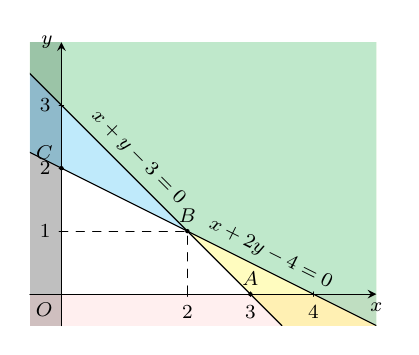
\begin{tikzpicture}[scale=0.8,font=\footnotesize,line join=round,line cap=round,>=stealth]
					\tikzset{every node/.style={scale=0.9}}
					\begin{scope}
						\clip (-0.5,-0.5) rectangle (5,4);
						\fill[black,opacity=0.25] (0,-0.5)--(-0.5,-0.5)--(-0.5,4)--(0,4)--cycle;
						\fill[pink,opacity=0.25] (-0.5,0)--(-0.5,-0.5)--(5,-0.5)--(5,0)--cycle;
						\fill[yellow,opacity=0.25] (-1.5,4.5)--(6,4.5)--(6,-3)--cycle;
						\fill[cyan,opacity=0.25] (-4.5,4.25)--(6,4.25)--(6,-1)--cycle;
						\fill (3,0) circle (1pt) node[above]{$A$};
						\fill (2,1) circle (1pt) node[above]{$B$};
						\fill (0,2) circle (1pt) node[above left]{$C$};
						\draw (-1,4)--(3.5,-0.5) node [pos=0.45, above, sloped] {$x+y-3=0$};
						\draw (-4,4)--(5,-0.5) node [pos=0.8, above, sloped] {$x+2y-4=0$};
					\end{scope}
					\draw[->] (-0.5,0)--(5,0) node[below]{$x$};
					\draw[->] (0,-0.5)--(0,4) node[left]{$y$};
					\draw (0,0) node[below left]{$O$};
					\foreach \x in {2,3,4}
					\draw[thin] (\x,1pt)--(\x,-1pt) node [below] {$\x$};
					\foreach \y in {1,2,3}
					\draw[thin] (1pt,\y)--(-1pt,\y) node [left] {$\y$};
					\draw[dashed,thin] (2,0)--(2,1)--(0,1);
			\end{tikzpicture}}
		\end{enumerate}
	}
\end{vd}
\begin{dang}{Ứng dụng}
	Để giải bài toán tìm phương án tối ưu ta, thực hiện các bước sau
	\begin{itemize}
		\item Bước 1: Đặt các ẩn $x$, $y$ cho các đại lượng cần tìm.
		\item Bước 2: Lập hệ các bất phương trình mô tả các điều kiện và mối quan hệ giữa các đại lượng.
		\item Bước 3: Xây dựng hàm mục tiêu cho giá trị mà ta muốn đạt giá trị tối ưu có dạng $F = ax + by$.
		\item Bước 4: Biểu diễn miền nghiệm của hệ bất phương trình ta được một đa giác. Tìm tọa độ các đỉnh của đa giác.
		\item Bước 5: Tính giá trị của biểu thức $F = ax + by$ tại cặp số $(x; y)$ là tọa độ các đỉnh của đa giác rồi so sánh các giá trị đó. Từ đó, kết luận được giá trị lớn nhất hay giá trị nhỏ nhất (phương án tối ưu) cần tìm.
	\end{itemize}
\end{dang}
\begin{vd}%[Dự án đề cương 3 khối NH24-25 Đợt 1-Nguyễn Tiến Liên]%[0D2V2-3]
	Có $3$ nhóm máy $A$, $B$, $C$ dùng để sản xuất ra $2$ loại sản phẩm $I$ và $II$. Để sản xuất một đơn vị sản phẩm mỗi loại phải lần lượt dùng các máy thuộc nhóm máy khác nhau. Số máy trong một nhóm và số máy từng nhóm cần thiết để sản xuất ra một đơn vị sản phẩm thuộc mỗi loại được cho trong bảng bên dưới
	\begin{center}
		\begin{tabular}{|c|c|w{c}{3.2 cm}|w{c}{3.2 cm}|}
			\hline
			\multirow{2}{3 cm}{\centering \arraybackslash Nhóm} & \multirow{2}{5 cm}{\centering \arraybackslash Số máy trong mỗi nhóm} &\multicolumn{2}{c|}{\makecell{Số máy trong từng nhóm\\ để sản xuất một đơn vị sản phẩm}}\\
			\cline{3-4}
			& & Loại $I$&Loại $II$\\
			\hline
			$A$&$10$ & $2$ &$2$ \\
			\hline
			$B$&$4$ & $0$ &$2$ \\
			\hline
			$C$&$12$ & $2$ &$4$ \\
			\hline
		\end{tabular}
	\end{center}
	Một đơn vị sản phẩm $I$ lãi $3\,000$ đồng, một đơn vị sản phẩm $II$ lãi $5\,000$ đồng. Hãy lập phương án sản xuất hai loại sản phẩm trên sao cho có lãi cao nhất.
	\loigiai{
		\immini{Gọi $x$ và $y$ lần lượt là số đơn vị sản phẩm loại $I$ và $II$ $(x,y\ge 0)$.\\
		Số tiền lãi của đơn vị này là $f(x,y)=3x+5y$ (nghìn đồng).\\
		Ta có hệ bất phương trình
		\[\heva{&2x+2y\le10\\&2y\le4\\&2x+4y\le 12\\&x,y\ge 0}\Leftrightarrow \heva{&x+y\le5\\&y\le2\\&x+2y\le 6\\&x,y\ge 0.}\qquad (*)\]
		Bài toán trở thành tìm giá trị lớn nhất của $f(x,y)=3x+5y$ trên miền nghiệm của hệ $(*)$.\\
		Miền nghiệm của hệ $(*)$ là ngũ giác $OABCD$ (kể cả biên).
	
		Ta có $O(0;0)$, $A(5;0)$, $B(4;1)$, $C(2;2)$, $D(0;2)$.\\
		Suy ra $f(0;0)=0$; $f(5;0)=15$; $f(4;1)=17$; $f(2;2)=16$; $f(0;2)=10$ (nghìn đồng).\\
		Do đó $f(x,y)=3x+5y$ lớn nhất khi $(x;y)=(4;1)$ tức là cần sản xuất $4$ sản phẩm $I$ và $1$ sản phẩm $II$ để thu về lợi nhuận cao nhất.}{
			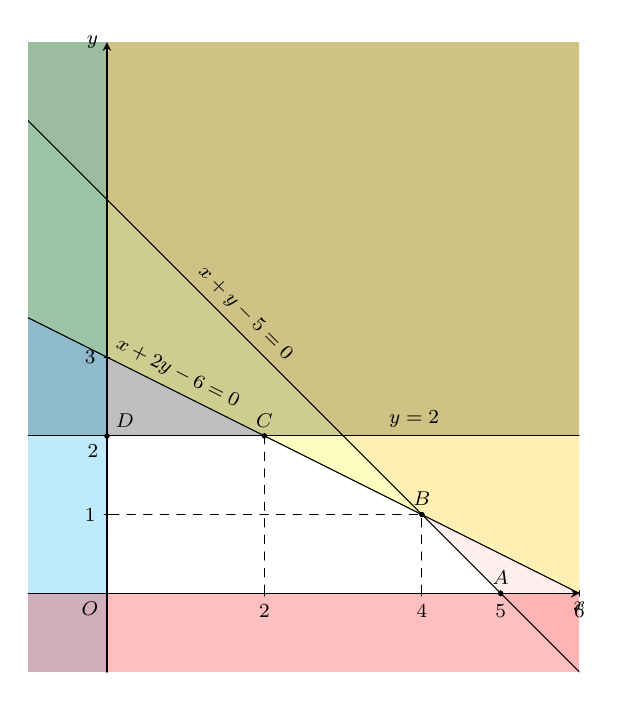
\begin{tikzpicture}[scale=1,font=\footnotesize,line join=round,line cap=round,>=stealth]
				\tikzset{every node/.style={scale=0.9}}
				\begin{scope}
					\clip (-1,-1) rectangle (6,7);
					\fill[pink,opacity=0.25] (-3,8)--(7,8)--(7,-2)--cycle;
					\fill[black,opacity=0.25] (-1,2)--(-1,7)--(6,7)--(6,2)--cycle;
					\fill[yellow,opacity=0.25] (-9,7.5)--(9,7.5)--(9,-1.5)--cycle;
					\fill[cyan,opacity=0.25] (0,-1)--(-1,-1)--(-1,7)--(0,7)--cycle;
					\fill[red,opacity=0.25] (-1,0)--(-1,-1)--(6,-1)--(6,0)--cycle;
					\fill (5,0) circle (1pt) node[above]{$A$};
					\fill (4,1) circle (1pt) node[above]{$B$};
					\fill (2,2) circle (1pt) node[above ]{$C$};
					\fill (0,2) circle (1pt) node[above right]{$D$};
					\draw (-2,7)--(6,-1) node [pos=0.45, above, sloped] {$x+y-5=0$};
					\draw (-1,2)--(6,2) node [pos=0.7, above, sloped] {$y=2$};
					\draw (-8,7)--(8,-1) node [pos=0.55, above, sloped] {$x+2y-6=0$};
				\end{scope}
				\draw[->] (-1,0)--(6,0) node[below]{$x$};
				\draw[->] (0,-1)--(0,7) node[left]{$y$};
				\draw (0,0) node[below left]{$O$};
				\foreach \x in {2,4,5,6}
				\draw[thin] (\x,1pt)--(\x,-1pt) node [below] {$\x$};
				\foreach \y in {1,3}
				\draw[thin] (1pt,\y)--(-1pt,\y) node [left] {$\y$};
				\draw(0,2)node[below left]{$2$};
				\draw[dashed,thin] (2,0)--(2,2)--(0,2);
				\draw[dashed,thin] (4,0)--(4,1)--(0,1);
			\end{tikzpicture}}
	}
\end{vd}
\begin{vd}%[Dự án đề cương 3 khối NH24-25 Đợt 1-Nguyễn Tiến Liên]%[0D2V2-3]
	Một hộ nông dân định trồng đậu và cà trên diện tích $800$ m$^2$. Nếu trồng đậu thì cần $20$ công và thu $3\,000\,000$ đồng trên $100$ m$^2$ nếu trồng cà thì cần $30$ công và thu $4\,000\,000$ đồng trên $100$ m$^2$. Hỏi cần trồng mỗi loại cây trên diện tích là bao nhiêu để thu được nhiều tiền nhất khi tổng số công không quá $180$.
	\loigiai{
			\immini{Gọi $x$, $y$ lần lượt là số m$^2$ đất trồng đậu, số m$^2$ đất trồng cà (đơn vị tính $100$ m$^2$; $x,y\ge 0$).\\
			Theo đề bài ta có
			$\heva{&x+y\le 8\\&20x+30y\le180\\&x\ge 0\\&y\ge 0}\Leftrightarrow \heva{&x+y\le 8\\&2x+30\le18\\&x\ge 0\\&y\ge 0.}$\\
			Miền nghiệm hệ bất phương trình là tứ giác $OABC$ với $A(0;6)$, $B(6;2)$, $C(8;0)$.\\
			Số tiền thu được là $T=3x+4y$ (triệu đồng).\\
			Suy ra $T(0;6)=24$, $T(6;2)=26$, $T(8;0)=24$,\\ $T(0;0)=0$ (triệu đồng).\\
			Vậy cần trồng $600$ m$^2$ đất trồng đậu và $200$ m$^2$ đất trồng cà để thu được nhiều tiền nhất.}{
		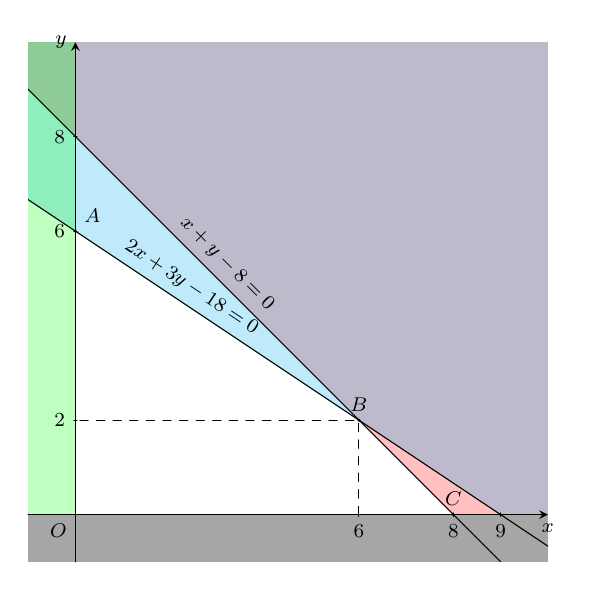
\begin{tikzpicture}[scale=0.6,font=\footnotesize,line join=round,line cap=round,>=stealth]
				\tikzset{every node/.style={scale=0.9}}
				\begin{scope}
					\clip (-1,-1) rectangle (10,10);
					\fill[red,opacity=0.25] (-3,11)--(11,11)--(11,-3)--cycle;
					\fill[cyan,opacity=0.25] (-7,10.67)--(11,10.67)--(11,-1.33)--cycle;
					\fill[green,opacity=0.25] (0,-1)--(-1,-1)--(-1,10)--(0,10)--cycle;
					\fill[black!35] (-1,0)--(-1,-1)--(10,-1)--(10,0)--cycle;
					\fill (0,6) circle (1pt) node[above right]{$A$};
					\fill (6,2) circle (1pt) node[above]{$B$};
					\fill (8,0) circle (1pt) node[above]{$C$};
					\draw (-2,10)--(9,-1) node [pos=0.45, above, sloped] {$x+y-8=0$};
					\draw (-6,10)--(10.5,-1) node [pos=0.5, above, sloped] {$2x+3y-18=0$};
				\end{scope}
				\draw[->] (-1,0)--(10,0) node[below]{$x$};
				\draw[->] (0,-1)--(0,10) node[left]{$y$};
				\draw (0,0) node[below left]{$O$};
				\foreach \x in {6,8,9}
				\draw[thin] (\x,1pt)--(\x,-1pt) node [below] {$\x$};
				\foreach \y in {2,6,8}
				\draw[thin] (1pt,\y)--(-1pt,\y) node [left] {$\y$};
				\draw[dashed,thin] (6,0)--(6,2)--(0,2);
		\end{tikzpicture}}
	}
\end{vd}
%-----------------------------------------------------------------------------
\subsection{Bài tập rèn luyện}
\ind{PHẦN I.} \inden{Câu trắc nghiệm nhiều phương án lựa chọn. Mỗi câu hỏi học sinh chỉ chọn một phương án.}\\
\setcounter{ex}{0}
\Opensolutionfile{ans}[ans/0D2-Bai2-TN]%--Đặt tên 0D2-Bai2-Dang1-TN
%câu 1
\begin{ex}[Lớp 10-GHKI NH24-25-THPT Tây Thạnh-TPHCM]%[Dự án đề cương 3 khối NH24-25 Đợt 1-Nguyễn Tiến Liên]%[0D2N2-2] 
	Miền nghiệm của hệ bất phương trình 
	$\heva{&x-2y<0 \\& x+3y >-2}$ không chứa điểm nào sau đây?
	\choice
	{\True $B(2 ; 1)$}
	{$D(0 ; 3)$}
	{$C(-3 ; 4)$}
	{$A(-1 ; 0)$}
	\loigiai{
		Thay $x=2$, $y=1$ vào
		$\heva{&x-2y<0 \\& x+3y >-2}$ ta được
		$\heva{&2-2\cdot 1<0 \\& 2+3\cdot 1 >-2}$ (mâu thuẫn).\\
		Vậy miền nghiệm của hệ bất phương trình 
		$\heva{&x-2y<0 \\& x+3y >-2}$ không chứa điểm $B(2 ; 1)$.
	}
\end{ex}
%câu 2
\begin{ex}[Lớp 10 GHKII NH24-25-THPT Nguyễn Thái Bình]%[Dự án đề cương 3 khối NH24-25 Đợt 1-Nguyễn Tiến Liên]%[0D2N2-1]
	Hệ bất phương trình nào sau đây là hệ bất phương trình bậc nhất hai ẩn?
	\choice
	{$\heva{&3x+y \leq 9 \\ &\frac{2}{x}-3y > 1}$}
	{$\heva{&3x^3-5y \geq 8 \\ &|-x-4y| \leq 20}$}
	{$\heva{&2x+3y^2 > 5 \\&-3x-5y \leq-6}$}
	{\True $\heva{&-3x+y \leq-1 \\ &4x-7y > 5}$}
	\loigiai{
		Ta có $\heva{&-3x+y \leq-1 \\ &4x-7y > 5}$ là hệ bất phương trình bậc nhất hai ẩn.	
	}
\end{ex}
%câu 3
\begin{ex}[Lớp 10 GHKII NH24-25-THPT Nguyen Thái Bình]%[Dự án đề cương 3 khối NH24-25 Đợt 1-Nguyễn Tiến Liên]%[0D2N2-1]
	Cho hệ bất phương trình $\heva{x-3y>5 \\2x+y<3.}$\\
	Cặp số $(x;y)$ nào sau đây là nghiệm của hệ bất phương trình trên?
	\choice
	{$(3;-1)$}
	{$(1;2)$}
	{$(3;1)$}
	{\True $(1;-2)$}
	\loigiai{
		Ta có $\heva{1-3\cdot (-2)=7>5\\2\cdot 1 + (-2)=0<3.}$\\
		Vậy cặp số $(1;-2)$ là nghiệm của hệ bất phương trình trên.
	}
\end{ex}
%câu 4
\begin{ex}%[Dự án đề cương 3 khối NH24-25 Đợt 1-Nguyễn Tiến Liên]%[0D2H2-2]
	Trong các cặp số sau, cặp số nào \textbf{không} là nghiệm của hệ bất phương trình $\heva{&x+y-2 \leq 0 \\ &2 x-3 y+2>0}$?
	\choice
	{$(0 ; 0)$}
	{$(1 ; 1)$}
	{\True $(-1 ; 1)$}
	{$(-1 ;-1)$}
	\loigiai{
		Ta thay cặp số $(-1 ; 1)$ vào hệ ta thấy không thỏa mãn.\\
		Vậy cặp số $(-1 ; 1)$ \textbf{không} là nghiệm của hệ bất phương trình $\heva{&x+y-2 \leq 0 \\ &2 x-3 y+2>0.}$
	}
\end{ex}
%câu 5
\begin{ex}%[Dự án đề cương 3 khối NH24-25 Đợt 1-Nguyễn Tiến Liên]%[0D2H2-2]
	Miền nghiệm của hệ bất phương trình $\heva{&\dfrac{x}{2}+\dfrac{y}{3}-1 \geq 0 \\ &2(x-1)+\dfrac{3 y}{2} \leq 4\\& x \geq 0}$ là phần mặt phẳng chứa điểm nào sau đây?
	\choice
	{\True $(2 ; 1)$}
	{$(0 ; 0)$}
	{$(1 ; 1)$}
	{$(3 ; 4)$}
	\loigiai{
		Ta có điểm $(2 ; 1)$ thỏa mãn hệ.
	}
\end{ex}
%câu 6
\begin{ex}%[Dự án đề cương 3 khối NH24-25 Đợt 1-Nguyễn Tiến Liên]%[0D2H2-2]
	Điểm nào sau đây \textbf{không} thuộc miền nghiệm của hệ bất phương trình $\heva{&2 x+3 y-1>0 \\& 5 x-y+4<0}$?
	\choice
	{$(-1 ; 4)$}
	{ $(-2 ; 4)$}
	{\True  $(0 ; 0)$}
	{ $(-3 ; 4)$}
	\loigiai{
		Ta có điểm $(0 ; 0)$ không thỏa mãn hệ.
	}
\end{ex}
%câu 7
\begin{ex}[Trích đề kiểm tra HKI-THPT - Chuyên Hùng Vương - Phú Thọ-NH-2024-2025]%[Dự án đề cương 3 khối NH24-25 Đợt 1-Nguyễn Tiến Liên]%[0D2H2-3]
	Một cửa hàng dự định kinh doanh hai loại máy điều hòa: điều hòa một chiều và điều hòa hai chiều. Khảo sát thị trường cửa hàng thấy nhu cầu của thị trường sẽ không vượt quá $100$ máy cả hai loại. Gọi $x$, $y$ lần lượt là số máy điều hòa một chiều và điều hòa hai chiều mà cửa hàng nhập vào. Khi đó, $(x; y)$ là nghiệm của hệ bất phương trình nào dưới đây?
	\choice
	{\True $\heva{&x \geq 0\\&y \geq 0\\&x + y \leq 100}$}
	{$\heva{&x \geq 0\\&y \geq 0\\&x + y < 100}$}
	{$\heva{&x \geq 0\\&y \geq 0\\&x + y \geq 100}$}
	{$\heva{&x \geq 0\\&y \geq 0\\&x + y > 100}$}
	\loigiai{
		Gọi $x$, $y$ lần lượt là số máy điều hòa một chiều và điều hòa hai chiều mà cửa hàng nhập vào.\\
		Điều kiện $x\geq 0$ và $y \geq 0$.\\
		Khảo sát thị trường cửa hàng thấy nhu cầu của thị trường sẽ không vượt quá $100$ máy cả hai loại nên ta có $x + y \leq 100$.\\
		Vậy hệ bất phương trình đúng là $\heva{&x \geq 0\\&y \geq 0\\&x + y \leq 100.}$
	}
\end{ex}
%câu 8
\begin{ex}%[Dự án đề cương 3 khối NH24-25 Đợt 1-Nguyễn Tiến Liên]%[0D2H2-2]
	Miền nghiệm của hệ bất phương trình $\heva{&x-y>0 \\ &x-3 y+3<0 \\ &x+y-5>0}$ là phần mặt phẳng chứa điểm
	\choice
	{\True $(5 ; 3)$}
	{ $(0 ; 0)$}
	{ $(1 ;-1)$}
	{$(-2 ; 2)$}
	\loigiai{
		Ta có điểm $(5 ; 3)$ thỏa mãn hệ.
	}
\end{ex}
%câu 9
\begin{ex}%[Dự án đề cương 3 khối NH24-25 Đợt 1-Nguyễn Tiến Liên]%[0D2H2-2]
	Miền nghiệm của hệ bất phương trình $\heva{&3 x+y \geq 9 \\ &x \geq y-3 \\ &2 y \geq 8-x \\ &y \leq 6}$ là phần mặt phẳng chứa điểm nào sau đây?
	\choice
	{$(0 ; 0)$}
	{$(1 ; 2)$}
	{$(2 ; 1)$}
	{\True $(8 ; 4)$}
	\loigiai{
		Ta có cặp số $(8 ; 4)$ thỏa bất phương trình $3 x+y \geq 9$.
	}
\end{ex}
%câu 10
\begin{ex}%[Dự án đề cương 3 khối NH24-25 Đợt 1-Nguyễn Tiến Liên]%[0D2H2-2]
	Cho hệ bất phương trình $\heva{&x+y>0 \\ &2 x+5 y<0}$ có tập nghiệm là $S$. Khẳng định nào sau đây là khẳng định đúng?
	\choice
	{$(1 ; 1) \in S$}
	{ $(-1 ;-1) \in S$}
	{\True  $\left(1 ;-\dfrac{1}{2}\right) \in S$}
	{ $\left(-\dfrac{1}{2} ; \dfrac{2}{5}\right) \in S$}
	\loigiai{
		Thế đáp án, chỉ có $x=1$ ; $y=-\dfrac{1}{2}$ thỏa mãn hệ bất phương trình.
	}
\end{ex}
%câu 11
\begin{ex}%[Dự án đề cương 3 khối NH24-25 Đợt 1-Nguyễn Tiến Liên]%[0D2H2-2]
	Miền nghiệm của hệ bất phương trình $\heva{&3 x+y \geq 6 \\ &x \geq y-3 \\ &2 y \geq 8-x \\ &y \leq 4}$ là phần mặt phẳng chứa điểm nào sau đây?
	\choice
	{$(2 ; 1)$}
	{\True  $(6 ; 4)$}
	{$(0 ; 0)$}
	{$(1 ; 2)$}
	\loigiai{
		Thế $x=6$; $y=4$ vào từng bất phương trình trong hệ, ta lần lượt có các mệnh đề đúng.\\
		Vậy ta chọn đáp án $(6; 4)$.\\
		Đáp án $(2;1)$ có toạ độ không thoả bất phương trình thứ $3$.
		Đáp án $(0;0)$, $(1;2)$ có tọa độ không thoả bất phương trình thứ $1$ và $3$
	}
\end{ex}
%câu 12
\begin{ex}[Lớp 10-THPT-HoangViet-DakLak-HKI-NH24-25]%[Dự án đề cương 3 khối NH24-25 Đợt 1-Nguyễn Tiến Liên]%[0D2H2-2]
\immini{Phần không gạch chéo ở hình bên là biểu diễn miền nghiệm của hệ bất phương trình nào dưới đây?
	\choice
	{\True $\heva{&y>0\\&3x+2y<6}$}
	{$\heva{&y>0\\&3x+2y<-6}$}
	{$\heva{& x>0\\&3x+2y<6}$}
	{$\heva{& x>0\\&3x+2y>-6}$}}{
	\begin{tikzpicture}[line join=round, line cap=round,>=stealth]
		\tikzset{every node/.style={scale=0.7}}
		\begin{scope}
			\clip (-2,-1) rectangle (4,5);
			\fill[pattern=north west lines,opacity=0.65] (-3,7.5)--(5,7.5)--(5,-4.5)--cycle;
			\fill[pattern=north west lines,opacity=0.65] (-2,0)--(-2,-1)--(4,-1)--(4,0)--cycle;
			\draw (-1.33,5)--(2.67,-1) node [pos=0.45, above, sloped] {~};
		\end{scope}
		\draw[->] (-2,0)--(4,0) node[below]{$x$};
		\draw[->] (0,-1)--(0,5) node[left]{$y$};
		\draw (0,0) node[below left]{$O$};
		\foreach \x in {2}
		\draw[thin] (\x,1pt)--(\x,-1pt) node [below] {$\x$};
		\foreach \y in {3}
		\draw[thin] (1pt,\y)--(-1pt,\y) node [left] {$\y$};
	\end{tikzpicture}
}
\loigiai{
	Chọn điểm $A(0;1)$ thuộc miền nghiệm của hệ bất phương trình thế vào các đáp án ta được đáp án đúng là $\left\{\begin{aligned}
		& y>0\\ 
		& 3x+2y<6\\ 
	\end{aligned}\right.$.}
	\end{ex}
%câu 13
\begin{ex}[Lớp 10-THPT-HoangViet-DakLak-HKI-NH24-25]%[Dự án đề cương 3 khối NH24-25 Đợt 1-Nguyễn Tiến Liên]%[0D2H2-3]
Ngoài giờ học, bạn Nam làm thêm việc phụ bán cơm được $15$ nghìn đồng/một giờ và phụ bán tạp hóa được $10$ nghìn đồng/một giờ. Nam không thể làm thêm việc nhiều hơn $15$ giờ mỗi tuần. Gọi $x$, $y$ lần lượt là số giờ phụ bán cơm và phụ bán tạp hóa. Hệ bất phương trình nào sau đây xác định số giờ để làm mỗi việc nếu Nam muốn kiếm được ít nhất $100$ nghìn đồng mỗi tuần?
\choice
{$\heva{&x \geq 0 \\& y \geq 0 \\& x+y \geq 15 \\& 15 x+10 y \geq 100}$}
{$\heva{&x \geq 0 \\& y \geq 0 \\& x+y \leq 15 \\& 15 x+10 y>100}$}
{\True $\heva{&x \geq 0 \\& y \geq 0 \\& x+y \leq 15 \\& 15 x+10 y \geq 100}$}
{$\heva{&x \geq 0 \\& y \geq 0 \\& x+y>15 \\& 15 x+10 y<100}$}
\loigiai{
	Gọi $x$, $y$ lần lượt là số giờ phụ bán cơm và phụ bán tạp hóa, tổng số giờ này không được nhiều hơn $15$ nên $x+y \leq 15$.\\
	Số tiền kiếm được sau $x$ giờ phục vụ cơm là $15x$.\\
	Số tiền kiếm được sau $y$ giờ bán tạp hóa là $10y$.\\
	Để Nam kiếm được ít nhất $100$ nghìn đồng mỗi tuần thì $15x+10y \geq 100$.\\
	Vậy ta có hệ $\heva{&x \geq 0 \\& y \geq 0 \\& x+y \leq 15 \\& 15 x+10 y \geq 100}$.
}
\end{ex}
%câu 14
\begin{ex}%[Dự án đề cương 3 khối NH24-25 Đợt 1-Nguyễn Tiến Liên]%[0D2H2-2]
	Miền tam giác $ABC$ kể cả ba cạnh sau đây là miền nghiệm của hệ bất phương trình nào trong bốn hệ bất phương trình dưới đây?
	\begin{center}
		\begin{tikzpicture}[scale=0.8,thick,>=stealth']
			%\fill[thin,color=gray!50] (-1,3.5) -- (4,3.5) -- (4,-1.2) -- (-1,2.8) -- cycle;
			%\fill[thin,color=gray!50] (-0.4,-3) -- (91/41,10/41) -- (4,-1.2) -- (4,-3) -- cycle;
			%\fill[thin,color=gray!50] (-1,2.8) -- (0,2) -- (0,-3) -- (-0.4,-3) --(-1,-3) -- cycle;
			\fill[thin,color=gray!50] (0,2) -- (0,-2.5) -- (91/41,10/41)  -- cycle;
			\draw[->] (-1,0) -- (4,0)node[above right]{$x$};
			\foreach \x in {1,2}
			\draw[shift={(\x,0)},color=black] (0pt,2pt) -- (0pt,-2pt) node[below] {\footnotesize $\x$};
			\draw[->,color=black] (0,-3) -- (0,3.5)node[above right]{$y$};
			\node[below right] at (0,0){$O$};
			\clip(-1,-3) rectangle (4,3.5);
			\draw[line width=1.2pt,smooth,samples=100,domain=-1:4] plot(\x,{5/4*(\x)-10/4});
			\draw[line width=1.2pt,smooth,samples=100,domain=-1:4] plot(\x,{10/5-4/5*(\x)});
			\foreach \y in {1,2,3}
			\draw[shift={(0,\y)},color=black] (2pt,0pt) -- (-2pt,0pt) node[left]{\footnotesize $\y$};
			\path
			(0,2) coordinate (A)
			(90/41,10/41) coordinate (B)
			(0,-2.5) coordinate (C)
			;
			\foreach \x/\g in {A/60,B/90,C/-10}
			\draw[fill=black] (\x) circle (.036)+(\g:.35)
			node{$\x$};
			\draw[shift={(2.5,0)},color=black] (0pt,2pt) -- (0pt,-2pt) node[below] {\footnotesize $\dfrac{5}{2}$};
		\end{tikzpicture}
	\end{center}
	\choice
	{$\heva{&y \geq 0 \\ &5 x-4 y \geq 10 \\ &5 x+4 y \leq 10}$}
	{$\heva{&x>0 \\ &5 x-4 y \leq 10 \\ &4 x+5 y \leq 10}$}
	{$\heva{&x \geq 0 \\ &4 x-5 y \leq 10 \\ &5 x+4 y \leq 10}$}
	{\True  $\heva{&x \geq 0 \\ &5 x-4 y \leq 10 \\ &4 x+5 y \leq 10}$}
	\loigiai{
		Cạnh $AC$ có phương trình $x=0$ và cạnh $AC$ nằm trong miền nghiệm nên $x \geq 0$ là một bất phương trình của hệ.\\
		Cạnh $AB$ qua hai điểm $\left(\dfrac{5}{2} ; 0\right)$ và $(0 ; 2)$ nên có phương trình $\dfrac{x}{\dfrac{5}{2}}+\dfrac{y}{2}=1 \Leftrightarrow 4 x+5 y=10$.\\
		Cạnh $BC$ qua hai điểm $(2 ; 0)$ và $\left(0;-\dfrac{5}{2}\right)$ nên có phương trình $\dfrac{x}{2}+\dfrac{y}{-\dfrac{5}{2}}=1 \Leftrightarrow 5x-4y=10$.\\
		Vậy hệ bất phương trình cần tìm là $\heva{&x \geq 0 \\ &5 x-4 y \leq 10 \\ &4 x+5 y \leq 10}$.
	}
\end{ex}
%câu 15
\begin{ex}%[Dự án đề cương 3 khối NH24-25 Đợt 1-Nguyễn Tiến Liên]%[0D2H2-2]
	Cho hệ bất phương trình $\heva{&x>0 \\ &x+\sqrt{3} y+1 \leq 0}$ có tập nghiệm là $S$. Khẳng định nào sau đây là khẳng định đúng?
	\choice
	{$(1 ;-1) \in S$}
	{$(1 ;-\sqrt{3}) \in S$}
	{\True  $(-1 ; \sqrt{5}) \notin S$}
	{$(-4 ; \sqrt{3}) \in S$}
	\loigiai{
		Ta thấy $(-1 ; \sqrt{5}) \notin S$ vì $-1<0$.
	}
\end{ex}
%câu 16
\begin{ex}%[Dự án đề cương 3 khối NH24-25 Đợt 1-Nguyễn Tiến Liên]%[0D2H2-2]
	Cho hệ bất phương trình $\heva{&x>0 \\ &x+\sqrt{3} y+1>0}$ có tập nghiệm là $S$. Khẳng định nào sau đây là khẳng định đúng?
	\choice
	{$(-1 ; 2) \in S$}
	{$(\sqrt{2} ; 0) \notin S$}
	{ $(1 ;-\sqrt{3}) \in S$}
	{\True $(\sqrt{3} ; 0) \in S$}
	\loigiai{
		Ta thấy $(\sqrt{3} ; 0) \in S$ vì $\heva{&\sqrt{3}>0 \\ &\sqrt{3}+\sqrt{3}\cdot0+1>0.}$
	}
\end{ex}
%câu 17
\begin{ex}%[Dự án đề cương 3 khối NH24-25 Đợt 1-Nguyễn Tiến Liên]%[0D2H2-2]
	Cho hệ bất phương trình $\heva{&x-y>3 \\& 1-\dfrac{1}{2} x+y>0}$ có tập nghiệm $S$. Khẳng định nào sau đây là khẳng định đúng?
	\choice
	{$(1 ;-2) \in S$}
	{$(2 ; 1) \in S$}
	{$(5 ;-6) \in S$}
	{\True $S=\varnothing$}
	\loigiai{
		Vì không có điểm nào thỏa hệ bất phương trình nên hệ bất phương trình đã cho có tập nghiệm $S=\varnothing$.
	}
\end{ex}
%câu 18
\begin{ex}%[Dự án đề cương 3 khối NH24-25 Đợt 1-Nguyễn Tiến Liên]%[0D2H2-2]
	Hệ bất phương trình $\heva{2 x-\dfrac{3}{2} y \geq 1 \\ 4 x-3 y \leq 2}$ có tập nghiệm $S$. Khẳng định nào sau đây là khẳng định đúng? 
	\choice
	{$\left(-\dfrac{1}{4} ;-1\right) \notin S$}
	{\True  $S=\{(x ; y) \mid 4 x-3 y=2\}$}
	{Biểu diễn hình học của $S$ là nửa mặt phẳng chứa gốc tọa độ và kể cả bờ $d$, với $d$ là là đường thẳng $4 x-3 y=2$}
	{Biểu diễn hình học của $S$ là nửa mặt phẳng không chứa gốc tọa độ và kể cả bờ $d$, với $d$ là đường thẳng $4 x-3 y=2$}
	\loigiai{
		\begin{center}
			\begin{tikzpicture}[scale=0.6,thick,>=stealth']
				\fill[gray,opacity=0.3] (-3,-3)--(-3,6) --(6,6)--(6,-3)-- cycle;
				\draw[->] (-3,0) -- (6,0)node[above]{$x$};
				\node[above left] at (0,0) {$O$};
				\clip(-3,-3) rectangle (6,6);
				\draw[->,color=black] (0,-3) -- (0,6)node[below right]{$y$};
				\draw[line width=1.2pt,smooth,samples=100,domain=-3:6] plot(\x,{(4/3)*(\x)-2/3});
				\draw[fill=black] (.5,0) circle (1pt) node[above]  {$\frac{1}{2}$};
				\draw[fill=black] (0,-2/3)circle (1pt)node[right] {$-\frac{2}{3}$};
			\end{tikzpicture}
		\end{center}
		Trước hết, ta vẽ đường thẳng $(d)\colon 4 x-3 y=2$.\\
		Thử trực tiếp ta thấy $(0 ; 0)$ là nghiệm của bất phương trình $4x-3y \leq 2$ nhưng không phải là nghiệm của phương trình $2x-\dfrac{3}{2}y\geq 1$.\\
		 Sau khi gạch bỏ các miền không thích hợp, tập hợp nghiệm của bất phương trình chính là các điểm thuộc đường thẳng $(d): 4 x-3 y=2$.
		
	}
\end{ex}
%câu 19
\begin{ex}%[Dự án đề cương 3 khối NH24-25 Đợt 1-Nguyễn Tiến Liên]%[0D2H2-2]
	Miền đa giác $ABCD$ ở hình bên dưới là miền nghiệm của hệ bất phương trình
	\begin{center}
	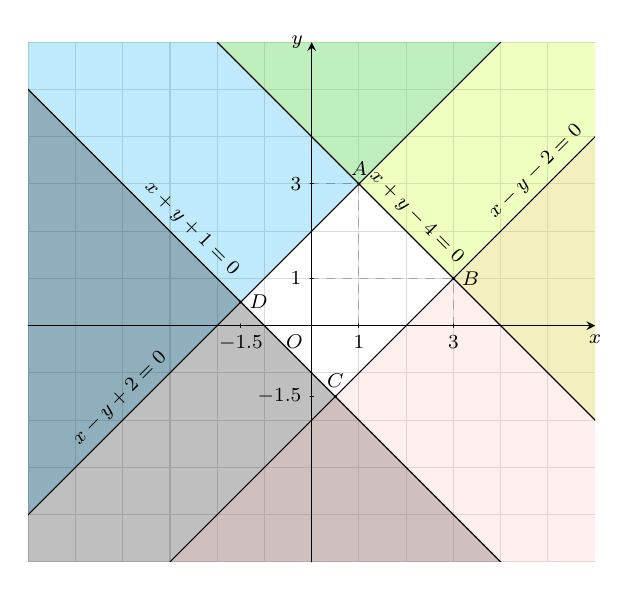
\begin{tikzpicture}[scale=0.6,font=\footnotesize,line join=round,line cap=round,>=stealth]
		\tikzset{every node/.style={scale=0.9}}
		\begin{scope}
			\clip (-6,-5) rectangle (6,6);
			\draw[opacity=0.15] (-6,-5) grid (6,6);			\fill[cyan,opacity=0.25](-6,6)--(-6,-4)--(4,6)--cycle;
			\fill[black,opacity=0.25] (-6,5)--(-6,-5)--(4,-5)--cycle;
			\fill[lime,opacity=0.25] (-2,6)--(10,-6)--(6,6)--cycle;
			\fill[pink,opacity=0.25] (-3,-5)--(6,-5)--(6,4)--cycle;
			\fill (1,3) circle (1pt) node[above]{$A$};
			\fill (-1.5,0.5) circle (1pt) node[right]{$D$};
			\fill (0.5,-1.5) circle (1pt) node[above]{$C$};
			\fill (3,1) circle (1pt) node[right]{$B$};
			\draw (-8,-6)--(4,6) node [pos=0.35, above, sloped] {$x-y+2=0$};
			\draw (-7,6)--(5,-6) node [pos=0.35, above, sloped] {$x+y+1=0$};
			\draw (-2,6)--(10,-6) node [pos=0.33, above, sloped] {$x+y-4=0$};
			\draw (-4,-6)--(8,6) node [pos=0.75, above, sloped] {$x-y-2=0$};
		\end{scope}
		\draw[->] (-6,0)--(6,0) node[below]{$x$};
		\draw[->] (0,-5)--(0,6) node[left]{$y$};
		\draw (0,0) node[below left]{$O$};
		\foreach \x in {-1.5,1,3}
		\draw[thin] (\x,1pt)--(\x,-1pt) node [below] {$\x$};
		\foreach \y in {-1.5,1,3}
		\draw[thin] (1pt,\y)--(-1pt,\y) node [left] {$\y$};
	\draw[dashed,thin,opacity=0.25] (3,0)--(3,1)--(0,1);
		\draw[dashed,thin,opacity=0.25] (1,0)--(1,3)--(0,3);
	\end{tikzpicture}
	\end{center}
	\choice 
	{\True $\heva{& x+y \le 4 \\& x+y \ge -1 \\& x-y \le 2 \\& x-y \ge -2.}$}
	{$\heva{&x-y \le 4 \\& x-y \ge -1 \\& x+y \le 2 \\& x+y \ge -2.}$}
	{$\heva{& x+y \le 1 \\& x+y \ge -4 \\& x-y \le 2 \\& x-y \ge -2.}$}
	{$\heva{&x-y \le 1 \\& x-y \ge -4 \\& x+y \le 2 \\& x+y \ge -2.}$}
	\loigiai{
		Ta thấy điểm $(1;2)$ thuộc miền đa giác $ABCD$ nên $(1;2)$ là một nghiệm của hệ bất phương trình cần tìm.\\
		Thay $x=1$, $y=2$ vào hệ bất phương trình $\heva{& x+y \le 4 \\& x+y \ge -1 \\& x-y \le 2 \\& x-y \ge -2}$ thì thấy điểm $(1;2)$ có tọa độ thỏa mãn tất cả các bất phương trình trong hệ.\\
		Vậy miền đa giác $ABCD$ là miền nghiệm của hệ bất phương trình $\heva{& x+y \le 4 \\& x+y \ge -1 \\& x-y \le 2 \\& x-y \ge -2.}$
	}
\end{ex}
%câu 20
\begin{ex}%[Dự án đề cương 3 khối NH24-25 Đợt 1-Nguyễn Tiến Liên]%[0D2V2-3]
	Giá trị nhỏ nhất của biểu thức $F = -x + y$ trên miền nghiệm của hệ bất phương trình
	$\heva{&-2x + y \le 2 \\& -x + 2y \ge 4 \\& x + y \le 5}$ là
	\choice 
	{$0$}
	{\True $1$}
	{$2$}
	{$3$}
	\loigiai{
		\begin{center}
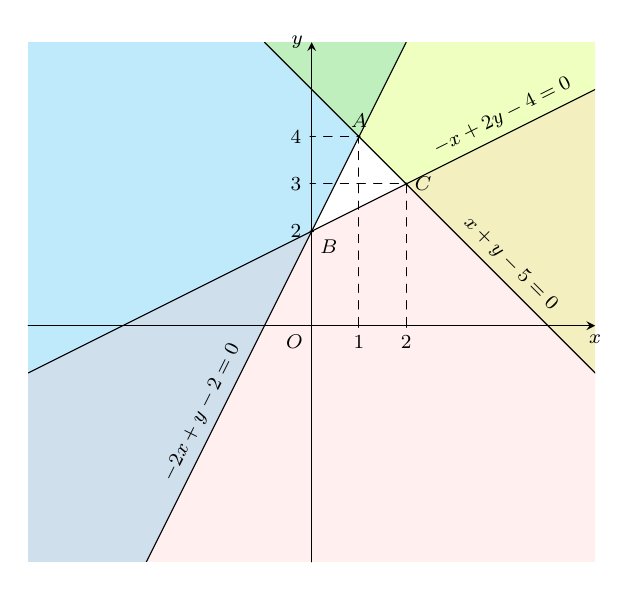
\begin{tikzpicture}[scale=0.6,font=\footnotesize,line join=round,line cap=round,>=stealth]
	\tikzset{every node/.style={scale=0.9}}
	\begin{scope}
		\clip (-6,-5) rectangle (6,6);
		\fill[cyan,opacity=0.25] (-6,-10)--(2,6)--(-6,6)--cycle;
		\fill[lime,opacity=0.25] (-1,6)--(6,-1)--(6,6)--cycle;
		\fill[pink,opacity=0.25] (-6,-1)--(-6,-5)--(6,-5)--(6,5)--cycle;
		\fill (1,4) circle (1pt) node[above]{$A$};
		\fill (0,2) circle (1pt) node[below right]{$B$};
		\fill (2,3) circle (1pt) node[right]{$C$};
		\draw (-6,-10)--(2,6) node [pos=0.5, above, sloped] {$-2x+y-2=0$};
		\draw (-6,-1)--(6,5) node [pos=0.85, above, sloped] {$-x+2y-4=0$};
		\draw (-1,6)--(10,-5) node [pos=0.45, above, sloped] {$x+y-5=0$};
	\end{scope}
	\draw[->] (-6,0)--(6,0) node[below]{$x$};
	\draw[->] (0,-5)--(0,6) node[left]{$y$};
	\draw (0,0) node[below left]{$O$};
	\foreach \x in {1,2}
	\draw[thin] (\x,1pt)--(\x,-1pt) node [below] {$\x$};
	\foreach \y in {2,3,4}
	\draw[thin] (1pt,\y)--(-1pt,\y) node [left] {$\y$};
	\draw[dashed,thin] (1,0)--(1,4)--(0,4);
	\draw[dashed,thin] (2,0)--(2,3)--(0,3);
\end{tikzpicture}
			\end{center}
			Miền nghiệm của hệ bất phương trình $\heva{&-2x + y \le 2 \\& -x + 2y \ge 4 \\& x + y \le 5}$ là miền tam giác $ABC$ kể cả bờ, với $A(1;4)$, $B(0;2)$, $C(2;3)$.\\
			$F(1;4)=3$, $F(0;2)=2$, $F(2;3)=1$.\\
			Vậy giá trị nhỏ nhất là $F=1$.
	}
\end{ex}

\Closesolutionfile{ans}

\ind{PHẦN II.} \inden{Câu trắc nghiệm đúng sai. Trong mỗi ý a), b), c), d) ở mỗi câu, học sinh chọn đúng hoặc sai.}\\
\setcounter{ex}{0}
\Opensolutionfile{ans}[ans/2D1-Bai1-DS]%--Đặt tên 2D1-Bai1-DS
%câu 1
\begin{ex}%[Dự án đề cương 3 khối NH24-25 Đợt 1-Nguyễn Tiến Liên]%[0D2H2-2]
	Cho hệ bất phương trình $\heva{&3x+2y\ge 9\\&x-2y\le 3\\&x+y\le 6\\&x\quad\ge 1}\,(I)$. Khi đó
	\choiceTF
	{Miền nghiệm của hệ bất phương trình là miền tam giác}
	{\True $(3;2)$ là một nghiệm của hệ bất phương trình}
	{$x=1$, $y=3$ là nghiệm của hệ bất phương trình $(I)$ sao cho $F=3x-y$ đạt giá trị lớn nhất}
	{\True $x=1$, $y=5$ là nghiệm của hệ bất phương trình $(I)$ sao cho $F=3x-y$ đạt giá trị nhỏ nhất}
	\loigiai{
		\begin{itemchoice}
			\itemch Miền nghiệm của hệ $(I)$ là miền tứ giác $ABCD$ với $A(3;0)$, $B(5;1)$, $C(1;5)$, $D(1;3)$ (Hình).\\
			\begin{center}
				\begin{tikzpicture}[line join=round, line cap=round,>=stealth,thick]
					\tikzset{every node/.style={scale=0.9}}
					\begin{scope}
						\clip (-3,-2) rectangle (7,7);
						\fill[pattern=north east lines] (-4,10.5)--(-4,-7.5)--(8,-7.5)--cycle;
						\fill[pattern=north west lines] (-4,-3.5)--(18,-3.5)--(18,7.5)--cycle;
						\fill[pattern=horizontal lines] (-4,10)--(9,10)--(9,-3)--cycle;
						\fill[pattern=vertical lines] (1,-2)--(-3,-2)--(-3,7)--(1,7)--cycle;
						\draw (-1.67,7)--(4.33,-2);% node [pos=0.45, above, sloped] {$3x+2y-9=0$};
						\draw (17,7)--(-1,-2);% node [pos=0.45, above, sloped] {$x-2y-3=0$};
						\draw (-1,7)--(8,-2);% node [pos=0.45, above, sloped] {$x+y-6=0$};
						\draw (1,-2)--(1,7);% node [pos=0.45, above, sloped] {$x-1=0$};
					\end{scope}
					\draw[->] (-3,0)--(7,0) node[inner sep=0.5pt,circle,fill=white,below]{$x$};
					\draw[->] (0,-2)--(0,7) node[inner sep=0.5pt,circle,fill=white,left]{$y$};
					\draw (0,0) node[inner sep=0.5pt,circle,fill=white,below left]{$O$};
					\foreach \x in {1,3,5,6}
					\draw[thin] (\x,1pt)--(\x,-1pt) node [inner sep=0.5pt,circle,fill=white,below] {$\x$};
					\foreach \y in {1,3,5,6}
					\draw[thin] (1pt,\y)--(-1pt,\y) node [inner sep=0.5pt,circle,fill=white,left] {$\y$};
					\draw[dashed,thin] (1,0)--(1,5)--(0,5);
					\draw[dashed,thin] (5,0)--(5,1)--(0,1);
					\draw (3,0) circle (1pt) node[above,xshift=3pt]{$A$} (5,1) circle (1pt) node[above,inner sep=0.5pt,circle,fill=white,xshift=3pt]{$B$} (1,5) circle (1pt) node[inner sep=0.5pt,circle,fill=white,right]{$C$} (1,3) circle (1pt) node[right]{$D$};
				\end{tikzpicture}
			\end{center}
			\itemch $(3;2)$ là một nghiệm của hệ bất phương trình.
			\itemch 
			 Ta có $F(x;y)=3x-y$.\\Khi đó
			\begin{itemize}
				\item $F(3;0)=3\cdot3-0=9$.
				\item $F(5;1)=3\cdot5-1=14$.
				\item $F(1;5)=3\cdot1-5=-2$.
				\item $F(1;3)=3\cdot1-3=0$.
			\end{itemize}
	     	Suy ra $F$ đạt giá trị lớn nhất bằng $14$ tại $x=5$, $y=1$.
			\itemch $F$ đạt giá trị nhỏ nhất bằng $-2$ tại $x=1$, $y=5$.
		\end{itemchoice}
	}
\end{ex}
%câu 2
\begin{ex}[Lớp 10 GHKI NH24-25-THPT Tân Bình - TP HCM]%[Dự án đề cương 3 khối NH24-25 Đợt 1-Nguyễn Tiến Liên]%[0D2V2-2]
	Bác Minh dự định quy hoạch $x$ sào đất trồng cà tím và $y$ sào đất trồng cà chua. Bác chỉ có không quá $9$ triệu đồng để mua hạt giống. Cho biết tiền mua hạt giống cà tím là $200\,000$ đồng/sào và $100\,000$ đồng/sào. Gọi $x$ là số sào đất trồng cà tím và $y$ là số sào đất trồng cà chua.
	\choiceTF
	{\True Hệ bất phương trình biểu diễn điều kiện của bài toán là $\heva{&2x+y\leq 90\\&x\geq 0\\&y\geq0.}$}
	{\True $\left(2;1\right)$ là một nghiệm của hệ bất phương trình biểu diễn điều kiện của bài toán}
	{Miền nghiệm của hệ bất phương trình biểu diễn điều kiện của bài toán là một miền tứ giác}
	{\True Biểu thức $L=3x-2y$ đạt giá trị lớn nhất là $M$ và giá trị nhỏ nhất là $m$. Khi đó $M-m=315$}
	\loigiai{
		\begin{itemchoice}
			\itemch Gọi $x$ là số sào đất trồng cà tím và $y$ là số sào đất trồng cà chua.\\
			 Ta có hệ bất phương trình
			$\heva{&200\,000x+100\,000y\leq 9\,000\,000\\&x\geq 0\\&y\geq0}$ hay $\heva{&2x+y\leq 90\\&x\geq 0\\&y\geq0.}$
			\itemch Thay $\left(2;1\right)$ vào hệ bất phương trình $\heva{&2x+y\leq 90\\&x\geq 0\\&y\geq0}$ ta thấy thoả mãn nên $\left(2;1\right)$ là một nghiệm của hệ bất phương trình biểu diễn điều kiện của bài toán.
			\itemch
			\begin{center}
				\begin{tikzpicture}[scale=1, font=\footnotesize, line join=round, line cap=round, >=stealth]
					\draw[->] (-1,0) -- (3.3,0)node[above]{$x$};
					\draw[->,color=black] (0,-1) -- (0,5.3)node[right]{$y$};
					\clip(-1,-1) rectangle (3,5);
					\fill[pattern=north east lines,opacity=0.75] (-5,-4) -- (-5,5) -- (5,5) -- (5,-4) -- cycle;
					\fill[white] (0,0) -- (2,0) -- (0,4)--cycle;
					\draw[violet,line width=2pt,samples=100] (0,0) -- (2,0) -- (0,4)--cycle;
					
					%\foreach \x in {-2,2,4}
					\draw[shift={(0,2)},color=black] (0pt,2pt) -- (0pt,-2pt) node[left] {$45$};
					\draw[shift={(0,4)},color=black] (0pt,2pt) -- (0pt,-2pt) node[left] {$90$};
					\draw[shift={(2,0)},color=black] (0pt,2pt) -- (0pt,-2pt) node[below] {$45$};
					\node[below left] at (0,0){$O$};
				\end{tikzpicture}
			\end{center} Miền nghiệm của hệ bất phương trình $\heva{&2x+y\leq 90\\&x\geq 0\\&y\geq0}$ là một tam giác.
			\itemch Ta có $L(x;y)=3x-2y$.\\Khi đó
			\begin{itemize}
				\item $L(0;0)=3\cdot0-2\cdot0=0$.
				\item $L(45;0)=3\cdot45-2\cdot0=135$.
				\item $L(0;90)=3\cdot0-2\cdot90=-180$.
			\end{itemize}
			Do đó $M=135$ và $m=-180$.\\ Vậy $M-m=135-(-180)=135+180=315$.
		\end{itemchoice}
	}
\end{ex}
%câu 3
\begin{ex}[Lớp 10 GHKI NH24-25-THPT Tây Thạnh]%[Dự án đề cương 3 khối NH24-25 Đợt 1-Nguyễn Tiến Liên]%[0D2H2-3]
	Cho hệ bất phương trình có miền nghiệm là miền tam giác không gạch chéo như hình.
	\begin{center}
		\begin{tikzpicture}[scale=1, font=\footnotesize, line join=round, line cap=round, >=stealth]
			\draw[->] (-1,0)--(0,0)node[below left]{$O$}--(6.05,0)node[right]{$x$};
			\draw[->] (0,-1)--(0,5.05)node[right]{$y$};
			\clip (-0.98,-0.98) rectangle (5.98,4.98);
			\filldraw[pattern = north east lines, pattern color = black,opacity=0.45] (-1,8/3)--(6,1/3)--(6,-1)--(-1,-1)--cycle;%Tô nền
			\filldraw[pattern = north west lines, pattern color = black,opacity=0.45] (5.34,-1)--(4/3,5)--(6,5)--(6,-1)--cycle;
			\filldraw[pattern = north east lines, pattern color = black,opacity=0.45] (-0.5,-1)--(2.5,5)--(-1,5)--(-1,-1)--cycle;
			\draw[dashed] (1,0)--(1,2)--(0,2)
			(4,0)--(4,1)--(0,1) (2,0)--(2,4)--(0,4)
			;
			\draw[thick,blue] (1,2)--(2,4)--(4,1)--cycle;
			\foreach \x in {1,2,4} \fill[black] (\x,0)node[below]{$\x$} circle(1pt);
			\foreach \y in {1,2,4} \fill[black] (0,\y)node[left]{$\y$} circle(1pt);
			\fill[black] (1,2)circle(1pt) (2,4)circle(1pt) (4,1)circle(1pt);
		\end{tikzpicture}
	\end{center}
	\choiceTF
	{\True Điểm $A(2;2)$ thuộc miền nghiệm của hệ bất phương trình đã cho}
	{Hệ bất phương trình đã cho $3$ cặp số $\left(x_0;y_0\right)$ (với $x_0$, $y_0\in\mathbb{Z}$) thoả mãn}
	{\True Điểm $B(3;3)$ không thuộc miền nghiệm của hệ bất phương trình đã cho}
	{Biểu thức $T=29x+5y$ đạt giá trị bé nhất trên miền nghiệm của hệ bất phương trình cho cho bằng $34$}
	\loigiai{
		\begin{center}
			\begin{tikzpicture}[scale=1, font=\footnotesize, line join=round, line cap=round, >=stealth]
				\draw[->] (-1,0)--(0,0)node[below left]{$O$}--(6.05,0)node[right]{$x$};
				\draw[->] (0,-1)--(0,5.05)node[right]{$y$};
				\clip (-0.98,-0.98) rectangle (5.98,4.98);
				\filldraw[pattern = north east lines, pattern color = black,opacity=0.45] (-1,8/3)--(6,1/3)--(6,-1)--(-1,-1)--cycle;%Tô nền
				\filldraw[pattern = north west lines, pattern color = black,opacity=0.45] (5.34,-1)--(4/3,5)--(6,5)--(6,-1)--cycle;
				\filldraw[pattern = north east lines, pattern color = black,opacity=0.45] (-0.5,-1)--(2.5,5)--(-1,5)--(-1,-1)--cycle;
				\draw[dashed] (1,0)--(1,2)--(0,2)
				(4,0)--(4,1)--(0,1) (2,0)--(2,4)--(0,4)
				;
				\draw[thick,blue] (1,2)--(2,4)--(4,1)--cycle;
				\foreach \x in {1,2,4} \fill[black] (\x,0)node[below]{$\x$} circle(1pt);
				\foreach \y in {1,2,4} \fill[black] (0,\y)node[left]{$\y$} circle(1pt);
				\fill[black] (1,2)node[above left]{$M$}circle(1pt) (2,4)node[right]{$N$}circle(1pt) (4,1)node[above right]{$P$}circle(1pt);
			\end{tikzpicture}
		\end{center}
		Gọi ba đỉnh của miền nghiệm lần lượt là $M(1;2)$, $N(2;4)$ và $P(4;1)$.\\
		Đường thẳng $MN$ đi qua $M$ và $N$ nên có phương trình $2x-y=0$.\\
		Đường thẳng $MP$ đi qua $M$ và $P$ nên có phương trình $x+3y=7$.\\
		Đường thẳng $PN$ đi qua $P$ và $N$ nên có phương trình $3x+2y=14$.\\
		Miền tam giác là miền nghiệm của hệ bất phương trình $\heva{&2x-y\ge0\\&3x+2y\le14\\&x+3y\ge7.}$
		\begin{itemchoice}
			\itemch Điểm $A(2;2)$ là một đỉnh của miền tam giác nên điểm $A$  thuộc miền nghiệm.
			\itemch Các điểm có toạ độ $\left(x_0;y_0\right)$ (với $x_0$, $y_0\in\mathbb{Z}$) thuộc miền tam giác $MNP$ là $(1;2)$, $(2;4)$, $(2;2)$, $(4;1)$.\\
			Thay $x=3;\,y=2$ vào hệ bất phương trình ta được  $\heva{&2\cdot3-2\ge0\text{ (thoả mãn)}\\&3\cdot3+2\cdot2\le14\text{ (thoả mãn)}\\&3+3\cdot2\ge7\text{ (thoả mãn)}}$.\\
			Thay $x=2;\,y=3$ vào hệ bất phương trình ta được  $\heva{&2\cdot2-2\ge0\text{ (thoả mãn)}\\&3\cdot2+2\cdot3\le14\text{ (thoả mãn)}\\&2+3\cdot3\ge7\text{ (thoả mãn)}}$.\\
			Suy ra có $6$ cặp số $\left(x_0;y_0\right)$ (với $x_0$, $y_0\in\mathbb{Z}$) thoả mãn.
			\itemch Ta có toạ độ điểm $B(3;3)$ không thoả mãn bất phương trình $3x+2y\le14$ nên không thuộc miền nghiệm của hệ bất phương trình đã cho.
			\itemch Tại điểm $M(1;2)$, ta có $T=29\cdot1+5\cdot2=39$.\\
			Tại điểm $N(2;4)$, ta có $T=29\cdot2+5\cdot4=78$.\\
			Tại điểm $P(4;1)$, ta có $T=29\cdot4+5\cdot1=121$.\\
			Suy ra $T_{\min}=39$.
		\end{itemchoice}	
	}
\end{ex}
%câu 4
	\begin{ex}[Lớp 10 GHKI NH24-25-THPT Chuyên Lê Hồng Phong - TPHCM]%[Dự án đề cương 3 khối NH24-25 Đợt 1-Nguyễn Tiến Liên]%[0D2V2-2]
		Cho hệ bất phương trình $\heva{&x \geq 0\\&y \geq 0\\&x+y \leq 2.}$
		\choiceTF
		{\True Điểm $O(0; 0)$ thuộc miền nghiệm của hệ bất phương trình đã cho}
		{Miền nghiệm của hệ bất phương trình chỉ chứa 3 nghiệm có tọa độ là các số nguyên}
		{\True Miền nghiệm của hệ bất phương trình là miền tam giác}
		{Giá trị lớn nhất của $F (x; y)=3x-4y$ với $(x; y)$ thuộc miền nghiệm của hệ bất phương trình là $5$}
		\loigiai{
			Miền nghiệm của hệ bất phương trình đã cho là miền tam giác $OAB$ kể cả $3$ cạnh với $O(0; 0)$, $A(2; 0)$, $B(0;2)$.
			\begin{center}
				\begin{tikzpicture}[scale=1, font=\footnotesize, line join=round, line cap=round, >=stealth]
					\def\xt{-3} \def\xp{4} \def\yd{-2}\def\yt{4} 
					\def\a{-2} \def\b{3} \def\c{-1} \def\d{3}
					\draw[step=1,gray, very thin,opacity=0.3] (\xt+0.1,\yd+0.1) grid (\xp-0.1,\yt-0.1);
					\clip (\xt+0.05,\yd+0.05) rectangle (\xp-0.05,\yt-0.05);
					%%-----
					\draw[smooth, domain=\xt-.2:\xp+.2] plot(\x,{-1*\x+2}) ;
					\fill[pattern=north west lines,pattern color =gray,opacity=0.5] (5,5)--(-5,5)--plot[domain=\xt:\xp](\x,{-1*\x+2})--cycle;
					\fill[pattern=north west lines,pattern color =gray,opacity=0.5] (5,0)--(-5,0)--(-5,-2)--(5,-2)--cycle;
					\fill[pattern=north west lines,pattern color =gray,opacity=0.5] (0,5)--(-3,5)--(-3,-2)--(0,-2)--cycle;
					%%-----
					\foreach \x in {\a,...,-1,1,2,...,\b} {\draw[ shift={(\x,0)}] (0pt,3pt) -- (0pt,-3pt) node[below] { $\x$};}
					\foreach \y in {\c,...,-1,1,2,...,\d} {\draw[ shift={(0,\y)}] (3pt,0pt) -- (-3pt,0pt) node[left] {$\y$};}
					\draw[->] (\xt-0.2,0)--(\xp-0.05,0);
					\draw (\xp-0.2,-0.1) node [below]{$x$};
					\draw[->] (0,\yd-0.2)--(0,\yt-0.05);
					\draw (0,\yt-0.2) node [left]{$y$};
					\draw (2,0)node[above]{$A$};
					\draw (0,2)node[above right]{$B$};
					\fill (0,0) circle (1.2pt);
					\draw (0.05,0.05) node[below left]{$O$};
				\end{tikzpicture}
			\end{center}
			\begin{itemchoice}
				\itemch Dựa vào miền nghiệm đã xác định, điểm $O(0; 0)$ thuộc miền nghiệm của hệ bất phương trình đã cho.
				\itemch Ta có $6$ điểm: $(0;2)$, $(0;1)$, $(0;0)$, $(1;0)$, $(2;0)$, $(1;1)$ đều thuộc miền nghiệm của hệ bất phương trình.
				\itemch Miền nghiệm của hệ bất phương trình là miền tam giác.
				\itemch Ta có tọa độ các đỉnh của miền nghiệm là $(0;2)$, $(0;0)$, $(2;0)$. \\
				Giá trị $F(2,0)=6$ là giá trị lớn nhất của $F(x,y)$.
		\end{itemchoice}}
	\end{ex}
	%câu 5
\begin{ex}[Lớp 10-HKI NH24-25-THPT - Chuyên Hùng Vương - Phú Thọ]%[Dự án đề cương 3 khối NH24-25 Đợt 1-Nguyễn Tiến Liên]%[0D2V2-2]
	Cho $(x;y)$ là nghiệm của hệ bất phương trình $\heva{&-2x+y\le 2\\ &x\le 5\\& y\le 4\\ &x+y \ge -1.}$
	\choiceTF
		{Miền nghiệm của hệ là miền tam giác (tính cả cạnh)}
	{\True Cặp số $(x;y)=(0;0)$ là nghiệm của hệ}
	{\True Biểu thức $F(x;y)=-x-y$ đạt giá trị lớn nhất bằng $1$}
	{Biểu thức $F(x;y)=-x-y$ đạt giá trị nhỏ nhất khi $x=5$; $y=-6$}
	\loigiai{
		\begin{center}
			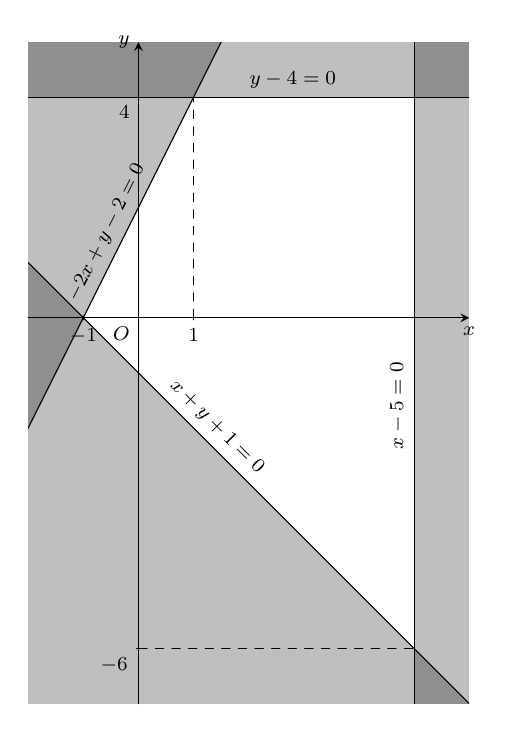
\begin{tikzpicture}[scale=0.7,line join=round,line cap=round,font=\footnotesize,>=stealth]
				\tikzset{every node/.style={scale=0.9}}
				\begin{scope}
					\clip (-2,-7) rectangle (6,5);
					\fill[black,opacity=0.25] (-5,-8)--(-5,16)--(7,16)--cycle;
					\fill[black,opacity=0.25] (5,-7)--(6,-7)--(6,5)--(5,5)--cycle;
					\fill[black,opacity=0.25] (-2,4)--(-2,5)--(6,5)--(6,4)--cycle;
					\fill[black,opacity=0.25] (-7,6)--(-7,-8)--(7,-8)--cycle;
					\draw (1.5,5)--(-4.5,-7) node [pos=0.3, above, sloped] {$-2x+y-2=0$};
					\draw (5,-7)--(5,5) node [pos=0.45, above, sloped] {$x-5=0$};
					\draw (-2,4)--(6,4) node [pos=0.6, above, sloped] {$y-4=0$};
					\draw (-6,5)--(6,-7) node [pos=0.6, above, sloped] {$x+y+1=0$};
				\end{scope}
				\draw[->] (-2,0)--(6,0) node[below]{$x$};
				\draw[->] (0,-7)--(0,5) node[left]{$y$};
				\draw (0,0) node[below left]{$O$};
				\draw(0,4)node[below left]{$4$};
				\foreach \x in {-1,1}
				\draw[thin] (\x,1pt)--(\x,-1pt) node [below] {$\x$};
				\foreach \y in {-6}
				\draw[thin] (1pt,\y)--(-1pt,\y) node [below left] {$\y$};
				\draw[dashed,thin] (1,0)--(1,4)--(0,4);
				\draw[dashed,thin] (5,0)--(5,-6)--(0,-6);
			\end{tikzpicture}
		\end{center}
		Miền nghiệm của hệ bất phương trình là miền tứ giác kể cả các cạnh có tọa độ các đỉnh là $A(1;4)$, $B(-1;0)$, $C(5;4)$, $D(5;-6)$.
		\begin{itemchoice}
			\itemch Miền nghiệm của hệ bất phương trình là miền tứ giác kể cả các cạnh.
			\itemch Thay tọa độ $(0;0)$ vào hệ bất phương trình ta thấy thỏa mãn.\\ Vậy $(x;y)=(0;0)$ là nghiệm của hệ.
			\itemch Ta có $F(1;4)=-5$, $F(-1;0)=1$, $F(5;4)=-9$, $F(5;-6)=1$.\\
			Vậy $F(x;y)$ đạt giá trị lớn nhất bằng $1$.
			\itemch Ta có $F(5;4)=-9$ là giá trị nhỏ nhất.\\
			Vậy $F(x;y)$ đạt giá trị nhỏ nhất khi $x=5; y=4$.
		\end{itemchoice}	}
\end{ex}
\Closesolutionfile{ans}
\ind{PHẦN III.} \inden{Câu trắc nghiệm trả lời ngắn}\\
\setcounter{ex}{0}
\Opensolutionfile{ans}[ans/2D1-Bai1-DS]%--Đặt tên 2D1-Bai1-DS
%câu 1
\begin{ex}%[Dự án đề cương 3 khối NH24-25 Đợt 1-Nguyễn Tiến Liên]%[0D3N1-3]
	Biểu thức $L=y-x$, với $x$ và $y$ thỏa mãn hệ bất phương trình $\heva{&3x+y-1 \leq 0\\&x\geq 0\\&2x-y-4\leq 0}$ đạt giá trị lớn nhất 
	là $a$ và đạt giá trị nhỏ nhất là $b$. Khi đó $a+12b$ bằng bao nhiêu?
	\shortans{$-47$}
	\loigiai{
			\begin{center}
			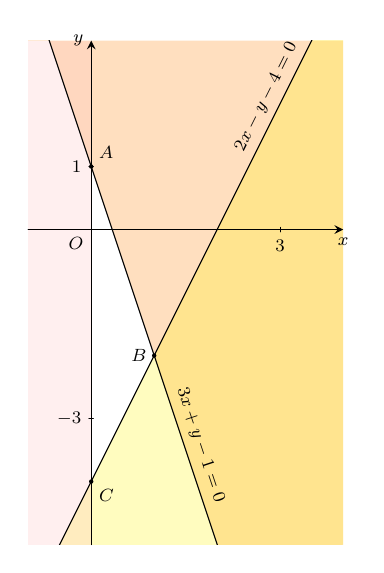
\begin{tikzpicture}[scale=0.8,font=\footnotesize,line join=round,line cap=round,>=stealth]
				\tikzset{every node/.style={scale=0.8}}
				\begin{scope}
					\clip (-1,-5) rectangle (4,3);
					\fill[orange,opacity=0.25] (-1,3)--(4,3)--(4,-11)--(-1,4)--cycle;
					\fill[yellow,opacity=0.25] (-1,-6)--(4,-5)--(4,3)--(4,4)--cycle;
					\fill[pink,opacity=0.25] (-1,-5)--(0,-5)--(0,3)--(-1,3)--cycle;
					\fill (0,1) circle (1pt) node[above right]{$A$};
					\fill (1,-2) circle (1pt) node[left]{$B$};
					\fill (0,-4) circle (1pt) node[below right]{$C$};
					\draw (-1,4)--(4,-11) node [pos=0.5, above, sloped] {$3x+y-1=0$};
					\draw (-1,-6)--(4,4) node [pos=0.8, above, sloped] {$2x-y-4=0$};
				\end{scope}
				\draw[->] (-1,0)--(4,0) node[below]{$x$};
				\draw[->] (0,-5)--(0,3) node[left]{$y$};
				\draw (0,0) node[below left]{$O$};
				\foreach \x in {3}
				\draw[thin] (\x,1pt)--(\x,-1pt) node [below] {$\x$};
				\foreach \y in {-3,1}
				\draw[thin] (1pt,\y)--(-1pt,\y) node [left] {$\y$};
			\end{tikzpicture}
		\end{center}
		Ta thấy $\left(0;0\right)$  là nghiệm của cả ba bất phương trình. Điều đó có nghĩa gốc tọa độ thuộc cả ba miền nghiệm của cả ba bất phương trình.
		Sau khi gạch bỏ các miền không thích hợp, miền không bị gạch là miền nghiệm của hệ (kể cả biên).\\
		Miền nghiệm là hình tam giác $ABC$  (kể cả biên), với các đỉnh: $A\left(0; 1\right), B\left(1; -2\right), C\left(0; -4\right)$.\\
		\begin{itemize}
			\item $L(A) = 1$.
			\item $L(B) = -3$.
			\item $L(C) = -4$.
		\end{itemize}
		Giá trị lớn nhất $a = 1$, giá trị nhỏ nhất $b = -4$.
		Khi đó $a+12b = -47$.
	}
\end{ex}
%câu 2
	\begin{ex}[Lớp 10-Thi giữa học kì 1 -Tây Thạnh-TPHCM]%[Dự án đề cương 3 khối NH24-25 Đợt 1-Nguyễn Tiến Liên]%[0D2V2-3]
	Bạn Linh đự định làm tối đa $9$ sản phẩm trang trí để bày bán tại gian hàng hội chợ của trường. Nếu làm một sản phẩm loại $A$ thì cần $40$ phút và thu được $15$ nghìn đồng. Nếu làm một sản phẩm loại $B$ thì cần $60$ phút và thu được $20$ nghìn đồng. Hãy tính số tiền nhiều nhất mà Linh có thế thu được (đơn vị nghìn đồng)? Biết bạn Linh chỉ có tối đa $8$ giờ cho việc làm các sản phẩm trang trí.
	
	\shortans{165}
	\loigiai{
		Gọi $x$ là số sản phẩm loại \( A \) mà Linh làm.\\
		Gọi $y$ là số sản phẩm loại \( B \) mà Linh làm. (điều kiện $x\geq 0$, $y\geq 0$.)\\
		Linh chỉ làm tối đa $9$ sản phẩm suy ra $x + y \leq 9$.\\
		Tổng thời gian làm sản phẩm không vượt quá $8$ giờ $=480$ phút.\\
		Suy ra $40x + 60y \leq 480\Leftrightarrow 2x + 3y \leq 24$.\\
		Lợi nhuận thu được (đơn vị: nghìn đồng) là $P = 15x + 20y$.\\
		Ta có hệ bất phương trình $\heva{&x+y \leq 9\\&2x+3y \leq 24\\&x \geq 0\\&y \geq 0.}$\\
		Biểu diễn các bất phương trình trên hệ trục tọa độ ta được miền nghiệm là miền trong của tứ giác $OABC$ kể cả các cạnh của tứ giác.
		\begin{center}
			\begin{tikzpicture}[line join=round, line cap=round,>=stealth,thick]
				\tikzset{label style/.style={font=\footnotesize}}
				\begin{scope}
					\clip (-2,-1) rectangle (13,10);
					\fill[pattern=north east lines,opacity=0.75] (-2,11)--(13,11)--(13,-1)--(10,-1);
					\fill[pattern=north east lines,opacity=0.75] (-2,9.33)--(13,9.33)--(13,-1)--(13.5,-1);
					\fill[pattern=north east lines,opacity=0.75] (0,-1)--(-2,-1)--(-2,10)--(0,10)--cycle;
					\fill[pattern=north east lines,opacity=0.75] (-1,0)--(-1,-1)--(13,-1)--(13,0)--cycle;
					\draw (-2,11)--(10,-1) node [pos=0.3, above, sloped] {$x+y=9$};
					\draw (-2,9.33)--(13.5,-1) node [pos=0.7, above, sloped] {$2x+3y=24$};
				\end{scope}
				\draw[->] (-3,0)--(13,0) node[below]{$x$};
				\draw[->] (0,-1)--(0,10) node[left]{$y$};
				\draw (0,0) node[below left]{$O$} (9,0)node[above right]{$A$} (3,6)node[above right]{$B$} (0,8)node[above right]{$C$};
				\draw[dashed](3,0)--(3,6)--(0,6);
				\foreach \x in {-2,-1,1,2,3,4,9,12}
				\draw[thin] (\x,1pt)--(\x,-1pt) node [below] {$\x$};
				\foreach \y in {1,2,3,4,5,6,8,9}
				\draw[thin] (1pt,\y)--(-1pt,\y) node [left] {$\y$};
			\end{tikzpicture}
		\end{center}
		\begin{itemize}
			\item Tại $O(0;0) \colon P = 15\cdot 0 + 20\cdot 0= 0$.
			\item Tại $A(9; 0) \colon P = 15\cdot 9 + 20\cdot 0 = 135 $.
			\item Tại $B(3; 6) \colon P = 15\cdot 3 + 20\cdot 6  = 165 $.
			\item Tại $C(0; 8) \colon P = 15\cdot 0 + 20\cdot 8 = 160 $.
		\end{itemize}
		Số tiền lớn nhất Linh thu được là $165$ nghìn đồng, khi làm $3$ sản phẩm loại $A$ và $6$ sản phẩm loại $B$.
	}
\end{ex}
%câu 3
\begin{ex}[Lớp 10 HKI NH24-25-THPT Chuyên Lê Hồng Phong- Tp HCM]%[Dự án đề cương 3 khối NH24-25 Đợt 1-Nguyễn Tiến Liên]%[0D2H2-3]
	Công ty TNHH A dự định sản xuất ít nhất $80$ kg đường vàng và $20$ kg đường trắng từ hai nguyên liệu là mía và củ cải. Từ một tạ mía giá $600$ ngàn đồng có thể sản xuất $40$ kg đường vàng và $5$ kg đường trắng. Từ một tạ củ cải giá $300$ ngàn đồng có thể sản xuất $8$ kg đường vàng và $4$ kg đường trắng. Nhưng nhà cung cấp nguyên liệu cho công ty chỉ còn $8$ tạ mía và $12$ tạ củ cải. Hỏi chi phí mua nguyên liệu của công ty ít nhất là bao nhiêu ngàn đồng?
	\par\shortans{$1\,800$}
	\loigiai{
		Gọi $x$ là số tạ mía cần mua, $y$ là số tạ củ cải cần mua. ($x,\, y \ge 0$)\\
		Số lượng đường vàng là $40x + 8y \ge 80$.\\
		Số lượng đường trắng là $5x + 4y \ge 20$.\\
		Giới hạn nguyên liệu là $x \le 8$; $y \le 12$.\\
		Chi phí mua nguyên liệu là $f(x;y) = 600x + 300y$.\\
		Bài toán trở thành: Tìm giá trị nhỏ nhất của biểu thức $f(x;y) = 600x + 300y$ với $(x;y)$ thoả mãn hệ bất phương trình
		$$\heva{&40x + 8y \ge 80\\&5x + 4y \ge 20\\&0\le x \le 8\\&0\le y \le 12.}$$
		Biểu diễn miền nghiệm của hệ bất phương trình ta được
		\begin{center}
			\begin{tikzpicture}[scale=0.6,>=stealth, font=\footnotesize, line join=round, line cap=round]
				\path (4/3,10/3) coordinate (A)
				(0,10) coordinate (B)
				(0,12) coordinate (C)
				(8,12) coordinate (D)
				(8,0) coordinate (E)
				(4,0) coordinate (F)
				(0,0) coordinate (O)
				;
				\draw[thick,->] (-1.1,0)--(10.2,0) node[below]{$x$};
				\draw[thick,->] (0,-1.1)--(0,13.1) node[right]{$y$};
				\clip (-0.95,-0.95) rectangle (9.95,12.95);
				\filldraw[pattern = north east lines, pattern color = black,opacity=0.45] (-1,-1)--(-1,13)--(10,13)--(10,-1)--cycle;
				\filldraw[white] (A)--(B)--(C)--(D)--(E)--(F)--cycle;
				\foreach \p/\g in {A/0, B/0, C/-60, D/-140, E/140, F/90, O/-140}
				\draw[fill=black] (\p) circle (1pt) node[shift=(\g:3mm)] {$\p$};
				\draw (-1.1,0)--(10.2,0) (0,-1.1)--(0,13.1);
				\draw[thick, samples=100,domain=-0.5:2.2] plot(\x,{10-5*(\x)});
				\draw[thick, samples=100,domain=-1:4.6] plot(\x,{5-1.25*(\x)});
				\draw[thick] (-1,12)--(10,12) (8,-1)--(8,13);
				\draw (F)node[below]{$4$} (B)node[left]{$10$} (C)node[above right]{$12$} 
				(E)node[below left]{$8$}
				;			
			\end{tikzpicture}
		\end{center}
		Miền nghiệm của hệ bất phương trình là miền lục giác $ABCDEF$ (kể cả biên) với $A\left(\dfrac{4}{3};\dfrac{10}{3}\right)$, $B(0;10)$, $C(0;12)$, $D(8;12)$, $E(8;0)$ và $F(4;0)$.\\
		Tính giá trị của $f(x;y)$ với $(x;y)$ tương ứng là toạ độ các điểm $A$, $B$, $C$, $D$, $E$, $F$ ta được $f(x;y)$ đạt giá trị nhỏ nhất bằng $1\,800$ tại $x=\dfrac{4}{3}$; $y=\dfrac{10}{3}$.\\
		Vậy chi phí mua nguyên liệu của công ty ít nhất là $1\,800$ ngàn đồng.
	}
\end{ex}
%câu 4
\begin{ex}%[Dự án đề cương 3 khối NH24-25 Đợt 1-Nguyễn Tiến Liên]%[0D2V2-2]
	Cho hệ bất phương trình $\heva{&x-y+4 \ge 0 \\& x+y \le 0 \\& x \le 0 \\& y+2 \ge 0}$. Miền nghiệm của hệ tạo thành đa giác có $n$ cạnh, với $n$ là số tự nhiên. Xác định $n$.
	\par\shortans{$4$}
	\loigiai{
		Biểu diễn miền nghiệm của hệ bất phương trình $\begin{cases} x-y+4 \ge 0 \\ x+y \le 0 \\ x \le 0 \\ y+2 \ge 0. \end{cases}$
		\begin{center}
			\begin{tikzpicture}[scale=.7,line join = round, line cap = round,>=stealth,font=\footnotesize]
				\draw[->] (-6,0)--(6,0) node[shift={(30:7pt)},font=\normalsize]{$x$};
				\draw[->] (0,-6)--(0,6) node[shift={(135:7pt)},font=\normalsize]{$y$};
				\path (0,0) node[shift={(225:9pt)}]{$O$}
				(-6,6) coordinate (M)
				(-6,-6) coordinate (N)
				(6,-6) coordinate (P)
				(6,6) coordinate (Q)
				(-6,-2)coordinate (A)
				(-2,2)coordinate (B)
				(0,-2)coordinate (C)
				;
				\clip (M) rectangle (P);
				\foreach \x in {-5,...,5}{
					\unless\ifnum\x=0
					\draw (\x,2pt)--(\x,-2pt) +(0,-7pt) node{$\x$};
					\fi
				}
				\foreach \y in {-2,-1,1,4}{
					\draw[fill=black] (0,\y)circle (1pt)node[below right]{$\y$};
				}
				
				\fill[pattern=north east lines,pattern color=black,opacity=0.5] plot[domain=-6:6](\x,{(1)*\x+4})--(M)--cycle;
				\path[draw=black] plot[domain=-6.1:5](\x,{(1)*\x+4});
				\path (-5,-1)--(5,9) node[sloped,pos=0.2,above]{$x-y+4=0$};
				\fill[pattern=north east lines,pattern color=black,opacity=0.5] plot[domain=-6:6](\x,{(-\x})--(Q)--cycle;
				\path[draw=black] plot[domain=-6:6](\x,{-\x});
				\path (M)--(P) node[sloped,pos=0.1,below]{$x+y=0$};
				\fill[pattern=north east lines,pattern color=black,opacity=0.5] (Q)--(0,6)--(0,-6)--(P)--cycle;
				\path[draw=black] (0,-5)--(0,5) node[sloped,pos=0.85,below]{};
				\fill[pattern=north east lines,pattern color=black,opacity=0.5] plot[domain=-6:6](\x,{-2})--(P)--(N)--cycle;
				\path[draw=black] plot[domain=-6.1:6](\x,{-2});
				\path (-5,-2)--(5,-2) node[sloped,pos=0.9,below]{$y+2=0$};
				\foreach \x/\g in {A/-39,B/-90,C/140}
				\draw (\x) circle (1.2pt)
				+(\g:8pt) node {$\x$};
			\end{tikzpicture}
		\end{center}
		Miền nghiệm của hệ là miền tứ giác $ABOC$ với $A(-6,-2)$, $B(-2,2)$ và $C(0,-2)$.\\
		Vậy $n=4$.
	}
\end{ex}
% Câu 5
\begin{ex}%[Dự án đề cương 3 khối NH24-25 Đợt 1-Nguyễn Tiến Liên]%[0D2V2-2]
	Cho biểu thức $T=3x-2y-4$ với $x$ và $y$ thỏa mãn hệ bất phương trình $\heva{& x-y-1\le 0 \\& x+4y+9\ge 0 \\& x-2y+3\ge 0}$. Biết $T$ đạt giá trị nhỏ nhất khi $x=x_0$ và $y=y_0$. Tính $x_0^2+y_0^2$.
	\par\shortans{$26$}
	\loigiai{
		Biểu diễn miền nghiệm của hệ bất phương trình  $\heva{& x-y-1\le 0 \\& x+4y+9\ge 0 \\& x-2y+3\ge 0.}$
		\begin{center}
			\begin{tikzpicture}[scale=.7,line join = round, line cap = round,>=stealth,font=\footnotesize]
				\draw[->] (-5.5,0)--(5.5,0) node[shift={(-85:7pt)},font=\normalsize]{$x$};
				\draw[->] (0,-5.5)--(0,5.5) node[shift={(175:7pt)},font=\normalsize]{$y$};
				\path (0,0) node[shift={(225:9pt)}]{$O$}
				(-5,5) coordinate (M)
				(-5,-5) coordinate (N)
				(5,-5) coordinate (P)
				(5,5) coordinate (Q)
				(-5,-1)coordinate (A)
				(-1,-2)coordinate (B)
				(5,4)coordinate (C)
				;
				\clip ($(N)-(0.25,0.25)$) rectangle ($(Q)+(0.75,0.75)$);
				\foreach \x in {-9,...,9}{\unless\ifnum\x=0
					\draw (\x,2pt)--(\x,-2pt) +(0,-7pt) node{$\x$};
					\fi
				}
				\foreach \y in {-9,...,9}{\unless\ifnum\y=0
					\draw (1pt,\y)--(-1pt,\y) +(10pt,0) node{$\y$};
					\fi
				}
				\fill[pattern=north east lines,pattern color=black,opacity=0.45] plot[domain=-5:5](\x,{(1)*\x-1})--(P)--cycle;
				\path[draw=black] plot[domain=-4:5](\x,{(1)*\x-1});
				\path (-5,-6)--(5,4) node[sloped,pos=0.775,below]{$x-y-1=0$};
				\fill[pattern=north east lines,pattern color=black,opacity=0.45] plot[domain=-5:5](\x,{(-1/4)*\x-9/4})--(P)--(N)--cycle;
				\path[draw=black] plot[domain=-5:5](\x,{(-1/4)*\x-9/4});
				\path (-5,-1)--(5,-7/2) node[sloped,pos=0.2,below]{$x+4y+9=0$};
				\fill[pattern=north east lines,pattern color=black,opacity=0.45] plot[domain=-5:5](\x,{(1/2)*\x+3/2})--(Q)--(M)--cycle;
				\path[draw=black] plot[domain=-5:5](\x,{(1/2)*\x+3/2});
				\path (-5,-1)--(5,4) node[sloped,pos=0.75,above]{$x-2y+3=0$};
				\foreach \x/\g in {A/-90,B/90,C/140} {\draw (\x) circle (1.2pt)+(\g:8pt) node {$\x$};}
			\end{tikzpicture}
		\end{center}
		Miền nghiệm của hệ là miền tam giác $ABC$ với $A(-5;-1)$, $B(-1;-2)$ và $C(5;4)$.\\
		Ta có bảng giá trị của $T$:
		\begin{center}
			\renewcommand{\arraystretch}{1.3}
			\begin{tabular}{|>{\centering\arraybackslash}m{2cm}|
					>{\centering\arraybackslash}m{2cm}|
					>{\centering\arraybackslash}m{2cm}|
					>{\centering\arraybackslash}m{2cm}|	}
				\hline
				Đỉnh & $A(-5;-1)$ & $B(-1;-2)$ & $C(5;4)$ \\
				\hline
				$T$ & $-17$ & $-3$ & $3$ \\
				\hline
			\end{tabular}
		\end{center}
		Vậy $T$ đạt giá trị nhỏ nhất bằng $-17$ khi $x=-5$ và $y=-1$.\\
		Do đó $x_0=-5$ và $y_0=-1 \Rightarrow x_0^2+y_0^2=(-5)^2+(-1)^2=25+1=26$.
	}
\end{ex}
\Closesolutionfile{ans}
\ind{PHẦN IV.} \inden{Tự luận.}\\
\setcounter{ex}{0}
%câu 1
\begin{ex}[Lớp 10-Đề thi HKI-NH24-25 - THPT Nguyễn Thái Bình-TPHCM]%[Dự án đề cương 3 khối NH24-25 Đợt 1-Nguyễn Tiến Liên]%[0D3V2-6]
	Một xưởng sản xuất đồ gỗ mỹ nghệ sản xuất ra hai bộ sản phẩm loại I và loại II. Mỗi bộ sản phẩm loại I  lãi $5$ triệu đồng, mỗi bộ sản phẩm loại II lãi $4$ triệu đồng. Để sản xuất mỗi bộ sản phẩm loại I cần máy làm việc trong $3$ giờ và nhân công làm việc trong $2$ giờ. Để sản xuất mỗi bộ sản phẩm loại II cần máy làm việc trong $3$ giờ và nhân công làm việc trong $1$ giờ. Biết rằng chỉ dùng máy hoặc chỉ dùng nhân công không thể đồng thời làm hai loại sản phẩm cùng lúc, số nhân công luôn ổn định. Một ngày máy làm việc không quá $15$ giờ, nhân công làm việc không quá $8$ giờ. Tính số tiền lãi (triệu đồng) lớn nhất xưởng đó đạt được trong một ngày.
	\loigiai{
		Gọi $x$ là số bộ sản phẩm loại I được sản xuất trong một ngày.\\
		Gọi $y$ là số bộ sản phẩm loại II được sản xuất trong một ngày.\\
		$x, y \in \mathbb{N^*}$.\\
		Số tiền lãi được tính theo công thức $L=5x+4y$ (triệu đồng).\\
		Từ đề bài ta có hệ bất phương trình sau
		$\heva{
			& 3x + 3y \leq 15 \\
			& 2x + y \leq 8 \\
			& x \geq 0 \\
			& y \geq 0.}$\\
		\begin{center}
			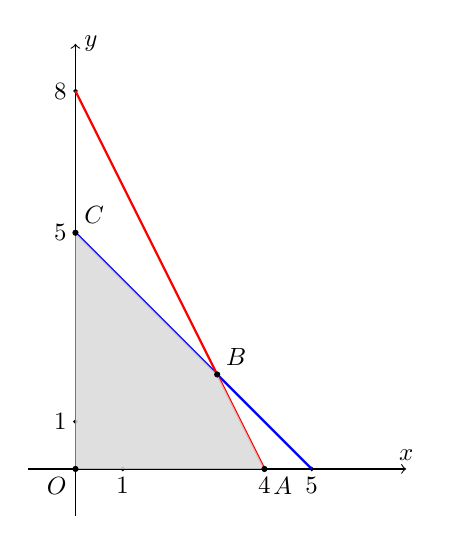
\begin{tikzpicture}[scale=0.6]
				% Vẽ hệ trục tọa độ
				\draw[->] (-1,0) -- (7,0) node[above] {$x$};
				\draw[->] (0,-1) -- (0,9) node[right] {$y$};
				\foreach \i in {1,5,8}{\draw[fill=black] (0,\i)circle (1pt)node[left]{$\i$};}
				\foreach \i in {1,4,5}{\draw[fill=black] (\i,0)circle (1pt)node[below]{$\i$};}
				% Vẽ các đường biên
				\draw[thick, blue] (0,5) -- (5,0);
				\draw[thick, red] (0,8) -- (4,0);
				
				% Tô màu miền nghiệm
				\fill[gray!30, opacity=0.85] (0,0) -- (0,5) -- (3,2) -- (4,0) -- cycle;
				
				% Ghi chú các điểm giao
				\filldraw[black] (0,5) circle (1.5pt) node[above right] {$C$};
				\filldraw[black] (3,2) circle (1.5pt) node[above right] {$B$};
				%\filldraw[black] (4,2) circle (1.5pt) node[above right] {$(4,2)$};
				\filldraw[black] (4,0) circle (1.5pt) node[below right] {$A$};
				\filldraw[black] (0,0) circle (1.5pt) node[below left] {$O$};
			\end{tikzpicture}
		\end{center}
		Miền nghiệm của hệ bất phương trình trên là tứ giác $OABC$ với $A(4;0)$, $B(3;2)$, $C(0;5)$.\\
		Từ đó $L(4;0)=20$, $L(0;0)=0$, $L(3;2)=23$, $L(0;5)=20$.\\
		Vậy tiền lãi lớn nhất xưởng đó đạt được trong một ngày là $23$ triệu đồng.
	}	
\end{ex}
%câu 2
\begin{ex}[Lớp 10-Đề thi GHKI-NH24-25-THPT Nguyễn Thị Minh Khai -TPHCM]%[Dự án đề cương 3 khối NH24-25 Đợt 1-Nguyễn Tiến Liên]%[0D2V2-3]
	Người ta dự định dùng hai loại nguyên liệu $K$, $P$ để sản xuất ít nhất $72$ kg sản phẩm loại $I$ và $80$ kg sản phẩm loại $II$. Từ mỗi tấn nguyên liệu $K$ giá $4$ triệu đồng, có thể sản xuất được $24$ kg sản phẩm loại $I$ và $40$ kg sản phẩm loại $II$. Từ mỗi tấn nguyên liệu $P$ giá $3$ triệu đồng, có thể sản xuất được $36$ kg sản phẩm loại $I$ và $20$ kg sản phẩm loại $II$. Hỏi phải dùng bao nhiêu tấn nguyên liệu mỗi loại để chi phí mua nguyên liệu là ít nhất? Biết rằng cơ sở cung cấp nguyên liệu chỉ có thể cung cấp tối đa $3$ tấn nguyên liệu loại $K$ và $4$ tấn nguyên liệu loại $P$.
	\loigiai{
		Gọi $x$, $y$ (tấn) lần lượt là số tấn nguyên liệu loại $K$ và $P$ cần mua. Khi đó $x \ge 0$, $y \ge 0$.\\
		Chi phí để mua $x$ tấn nguyên liệu $K$ và $y$ tấn nguyên liệu $P$ là $F(x;y)=4x+3y$ (triệu  đồng).\\
		Vì cơ sở cung cấp nguyên liệu chỉ có thể cung cấp tối đa $3$ tấn nguyên liệu loại $K$ và $4$ tấn nguyên liệu loại $P$ nên $x \le 3$, $y \le 4$.\\
		Vì cần sản xuất ít nhất $72$ kg sản phẩm loại $I$ và $80$ kg sản phẩm loại $II$ nên $24x+36y \ge 72$, $40x+20y \ge 80$.\\
		Từ đó ta thu được hệ bất phương trình sau
		$$\heva{&0\le x \le 3\\&0\le y \le 4\\&24x+36y \ge 72\\&40x+20y \ge 80} \Leftrightarrow \heva{&0\le x \le 3\\&0\le y \le 4\\&2x+3y \ge 6\\&2x+y \ge 4.}$$
		Biểu diễn miền nghiệm của hệ bất phương trình trên mặt phẳng tọa độ, miền nghiệm là phần trong của tứ giác $ABCD$ (kể cả các cạnh của tứ giác) với $A(0;4)$, $B(3;4)$, $C(3;0)$ và $D(1;1{,}5)$.
		\begin{center}
			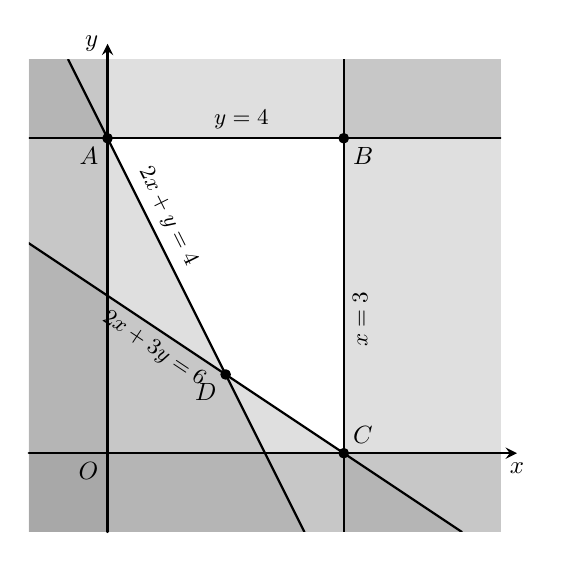
\begin{tikzpicture}[line join=round, line cap=round,>=stealth,thick]
				\tikzset{every node/.style={scale=0.9}}
				\begin{scope}
					\clip (-1,-1) rectangle (5,5);
					\fill[gray,opacity=0.25] (-5,5.33)--(-5,-2)--(6,-2)--cycle;
					\fill[gray,opacity=0.25] (-2,8)--(-2,-8)--(6,-8)--cycle;
					\fill[gray,opacity=0.25] (3,-1)--(5,-1)--(5,5)--(3,5)--cycle;
					\fill[gray,opacity=0.25] (-1,4)--(-1,5)--(5,5)--(5,4)--cycle;
					\fill[gray,opacity=0.25] (0,-1)--(-1,-1)--(-1,5)--(0,5)--cycle;
					\fill[gray,opacity=0.25] (-1,0)--(-1,-1)--(5,-1)--(5,0)--cycle;
					\draw (-4.5,5)--(4.5,-1) node [pos=0.58, below, sloped] {\small $2x+3y=6$};
					\draw (-0.5,5)--(2.5,-1) node [pos=0.35, above, sloped] {\small $2x+y=4$};
					\draw (3,-1)--(3,5) node [pos=0.45, below, sloped] {\small $x=3$};
					\draw (-1,4)--(5,4) node [pos=0.45, above, sloped] {\small $y=4$};
				\end{scope}
				\draw[->] (-1,0)--(5.2,0) node[below]{$x$};
				\draw[->] (0,-1)--(0,5.2) node[left]{$y$};
				\draw (0,0) node[below left]{$O$};
				\draw[fill=black] (0,4)circle(1.5pt) node[below left]{$A$}
				(3,4)circle(1.5pt) node[below right]{$B$}
				(3,0)circle(1.5pt) node[above right]{$C$}
				(1.5,1)circle(1.5pt) node[below left]{$D$}
				;
			\end{tikzpicture}
		\end{center}
		Ta có $F(0;4)=12$, $F(3;4)=24$, $F(3;0)=12$ và $F(1;1{,}5)=8{,}5$.\\
		 Nên giá trị nhỏ nhất cần tìm là $F(1;1{,}5)=8{,}5$.\\
		Vậy dùng $1$ tấn nguyên liệu loại $K$ và $1{,}5$ tấn nguyên liệu loại $P$ thì chi phí mua nguyên liệu là ít nhất.
	}
\end{ex}
%câu 3
\begin{ex}%[Dự án đề cương 3 khối NH24-25 Đợt 1-Nguyễn Tiến Liên]%[0D2V2-3]
	Một nhà máy có hai máy $A$, $B$ sản xuất mì tôm và miến gạo. Một tấn mì tôm lãi $3$ triệu đồng, một tấn miến gạo lãi $2{,}8$ triệu đồng. Muốn sản xuất $1$ tấn mì tôm dùng máy $A$ trong $3$ giờ và máy $B$ trong $1$ giờ. Muốn sản xuất $1$ tấn miến gạo dùng máy $A$ trong $1$ giờ và máy $B$ trong $1$ giờ. Một máy không thể dùng để sản xuất đồng thời cả mì tôm và miến gạo. Máy $A$ làm việc không quá $6$ giờ trong một ngày, máy $B$ một ngày chỉ làm việc không quá $4$ giờ. Hỏi muốn đạt số tiền lãi cao nhất thì  mỗi ngày nhà máy phải sản xuất bao nhiêu tấn mì tôm và bao nhiêu tấn miến gạo?
	\loigiai{
		Gọi $x$, $y$ lần lượt là số tấn mì tôm và miến gạo ($x\ge 0$, $y\ge 0$).\\
		Theo giả thiết suy ra hệ bất phương trình $\heva{&x\ge 0\\&y\ge 0&\\&3x+y\le 6\\&x+y\le 4.} (*)$\\
		\begin{center}
			\begin{tikzpicture}[scale=1.1, font=\footnotesize, line join=round, line cap=round, >=stealth]
				\begin{scope}
					\clip (-1,-1) rectangle (5,5);
					\fill[pattern=north east lines,opacity=0.4] (0,-1)--(-1,-1)--(-1,5)--(0,5)--cycle;
					\fill[pattern=north east lines,opacity=0.4] (-1,0)--(-1,-1)--(5,-1)--(5,0)--cycle;
					\fill[pattern=north east lines,opacity=0.4] (-2,12)--(6,12)--(6,-12)--cycle;
					\fill[pattern=north east lines,opacity=0.4] (-2,6)--(6,6)--(6,-2)--cycle;
					\draw (0.33,5)--(2.33,-1) node [pos=0.65, above, sloped] {$3x+y-6=0$};
					\draw (-1,5)--(5,-1) node [pos=0.45, above, sloped] {$x+y-4=0$};
					\draw[fill] (0,4) circle(1pt)  (1,3) node [left] {$B$} circle(1pt) (2,0) node [above left] {$C$} circle(1pt);
					\draw (0.1,3.9) node [below] {$A$};
				\end{scope}
				\draw[->] (-1,0)--(5,0) node[below]{$x$};
				\draw[->] (0,-1)--(0,5) node[left]{$y$};
				\draw (0,0) node[below left]{$O$};
				\foreach \x in {1,2,4}
				\draw[thin] (\x,1pt)--(\x,-1pt) node [below] {$\x$};
				\foreach \y in {3,4}
				\draw[thin] (1pt,\y)--(-1pt,\y) node [left] {$\y$};
			\end{tikzpicture}
		\end{center}
		Biểu diễn miền nghiệm của hệ $(*)$ ta được miền nghiệm của hệ $(*)$ là tứ giác $OABC$ trong đó $O(0;0)$, $A(0;4)$, $B(1;3)$, $C(2;0)$.\\
		Số tiền lãi mỗi ngày là $T(x;y)=3x+2{,}8y$ (triệu đồng).\\
		Thay tọa độ điểm $O$, $A$, $B$, $C$ vào biểu thức $T$.\\
		Ta có $T(0;0)=0$, $T(0;4)=11{,}2$, $T(1;3)=11{,}4$, $T(2;0)=6$.\\
		Vậy số tiền lãi cao nhất là $T=11{,}4$ triệu đồng khi mỗi ngày sản xuất $1$ tấn mì tôm và $3$ tấn miến gạo.
	}
\end{ex}
%câu 4
\begin{ex}%[Dự án đề cương 3 khối NH24-25 Đợt 1-Nguyễn Tiến Liên]%[0D2V2-2]
	Tìm giá trị lớn nhất của $f(x,y)=x+2y$ với điều kiện $\heva{&0\le y\le 4&  (d_1) \\& 0\le x & (d_2) \\& x-y-1\le 0 & (d_3) \\& x+2y-10\le 0 &(d_4).}$ $\quad (I)$
	\loigiai{
		Biểu diễn miền nghiệm của hệ bất phương trình $\heva{&0\le y\le 4 & (d_1) \\& 0\le x & (d_2) \\& x-y-1\le 0 & (d_3) \\& x+2y-10\le 0 & (d_4).}$ $\quad (I)$
		\begin{center}
			\begin{tikzpicture}[scale=.85,line join = round, line cap = round,>=stealth,font=\footnotesize]
				\draw[->] (-5,0)--(5,0) node[shift={(-85:7pt)},font=\normalsize]{$x$};
				\draw[->] (0,-5)--(0,5) node[shift={(175:7pt)},font=\normalsize]{$y$};
				\path (0,0) node[shift={(45:9pt)}]{$O$}
				(-5,5) coordinate (M)
				(-5,-5) coordinate (N)
				(5,-5) coordinate (P)
				(5,5) coordinate (Q)
				(1,0)coordinate (A)
				(4,3)coordinate (B)
				(2,4)coordinate (C)
				(0,4)coordinate (D)
				;
				\clip (M) rectangle (P);
				\foreach \x in {-4,...,4}{
					\unless\ifnum\x=0
					\draw (\x,2pt)--(\x,-2pt) +(0,-7pt) node{$\x$};
					\fi
				}
				\foreach \y in {-4,...,4}{	\unless\ifnum\y=0	\draw (2pt,\y)--(-2pt,\y) +(-5pt,0) node[above]{$\y$};
					\fi
				}
				\fill[pattern=north east lines,pattern color=black,opacity=0.65] plot[domain=-5:5](\x,{0})--(P)--(N)--cycle;
				\path[draw=black] plot[domain=-5:5](\x,{0});
				\path (-5,0)--(5,0) node[sloped,pos=0.25,below]{};
				\fill[pattern=north east lines,pattern color=black,opacity=0.65] plot[domain=-5:5](\x,{+4})--(Q)--(M)--cycle;
				\path[draw=black] plot[domain=-5:2.5](\x,{+4});
				\path (-5,4)--(5,4) node[sloped,pos=0.25,above]{$y=4$};
				\fill[pattern=north east lines,pattern color=black,opacity=0.65] (M)--(0,5)--(0,-5)--(N)--cycle;
				\path[draw=black] (0,-5.5)--(0,5.25) node[sloped,pos=0.85,above]{};
				\fill[pattern=north east lines,pattern color=black,opacity=0.65] plot[domain=-5:5](\x,{(1)*\x-1})--(P)--cycle;
				\path[draw=black] plot[domain=-5:5](\x,{(1)*\x-1});
				\path (-5,-6)--(5,4) node[sloped,pos=0.75,below]{$x-y-1=0$};
				\fill[pattern=north east lines,pattern color=black,opacity=0.65] plot[domain=-5:5](\x,{(-1/2)*\x+5})--(Q)--cycle;
				\path[draw=black] plot[domain=-5:5](\x,{(-1/2)*\x+5});
				\path (-5,15/2)--(5,5/2) node[sloped,pos=0.75,above]{$x+2y-10=0$};
				\foreach \x/\g in {A/90,B/190,C/-90,D/-50}	\draw[fill=black] (\x) circle (1pt)+(\g:10pt) node {$\x$};
			\end{tikzpicture}
		\end{center}
		$M(x;y)$ thỏa mãn hệ $(I)$ là miền bên trong ngũ giác $OABCD$.\\
		Trong đó $O(0;0)$, $A(1;0)$, $B(4;3)$, $C(2;4)$, $D(0;4)$.\\
		Thay tọa độ $O$, $A$, $B$, $C$, $D$ vào $f(x;y)=x+2y$ ta có bảng giá trị của $f(x;y)$, ta được
		\begin{center}
			\renewcommand{\arraystretch}{1.3}
			\begin{tabular}{|>{\centering\arraybackslash}m{2cm}|
					>{\centering\arraybackslash}m{2cm}|
					>{\centering\arraybackslash}m{2cm}|
					>{\centering\arraybackslash}m{2cm}|
					>{\centering\arraybackslash}m{2cm}|
					>{\centering\arraybackslash}m{2cm}|
				}
				\hline
				Đỉnh & $O$ & $A$ & $B$ & $C$ & $D$ \\
				\hline
				$f(x;y)$ & $0$ & $1$ & $10$ & $10$ & $8$ \\
				\hline
			\end{tabular}
		\end{center}
		Vậy giá trị lớn nhất của $f(x,y)=x+2y$ bằng $10$.
	}
\end{ex}
% Câu 5
\begin{ex}%[Dự án đề cương 3 khối NH24-25 Đợt 1-Nguyễn Tiến Liên]%[0D2V2-2]
	Với mọi cặp số $(x;y)$ thỏa mãn hệ bất phương trình 
	$\heva{&
		-2x+y \le 2 \\&
		-x+2y \le 4 \\&
		x+y \le 5 \\&
		y \ge 0.}$
		\\Có bao nhiêu giá trị nguyên của tham số $m$ trong $[-20;20]$ để $m \le -x+y$?
	\loigiai{
		\immini{Biểu diễn miền nghiệm của hệ bất phương trình
		$\heva{&-2x+y \le 2 \\&-x+2y \le 4 \\&x+y \le 5 \\&y \ge 0.}$\\
		Miền nghiệm của hệ bất phương trình là miền tứ giác $ABCD$ với $A(-1;0)$, $B(5;0)$, $C(2;3)$, $D(0;2)$.\\
		Ta có $x-y+m \le 0 \Leftrightarrow m\le -x+y$.}{
			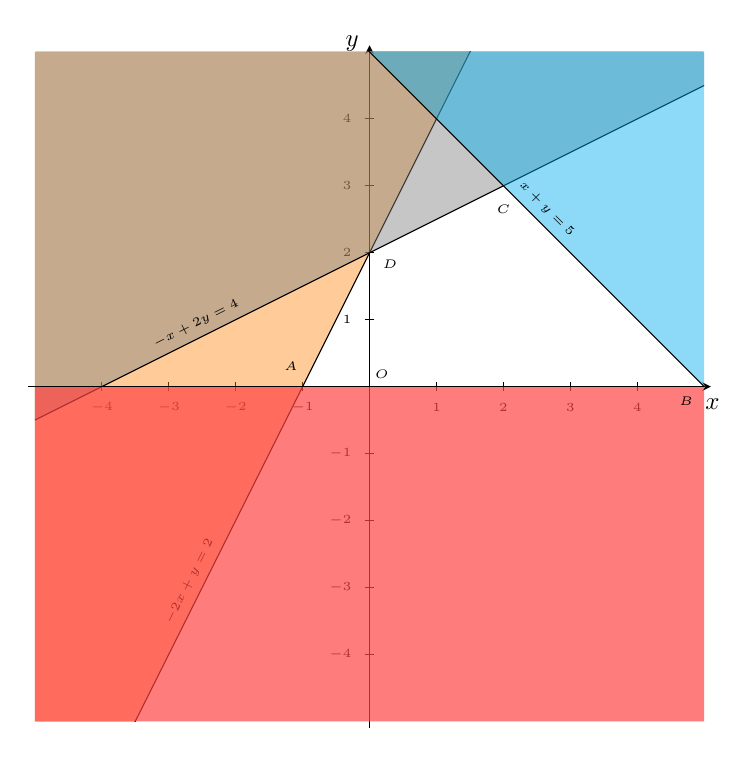
\begin{tikzpicture}[>=stealth,scale=0.85,font=\tiny]
				\draw[->] (-5.1,0)--(5.1,0) node[shift={(-85:7pt)},font=\normalsize]{$x$};
				\draw[->] (0,-5.1)--(0,5.1) node[shift={(175:7pt)},font=\normalsize]{$y$};
				\path (0,0) node[shift={(45:7pt)}]{$O$}
				(-5,5) coordinate (M) (-5,-5) coordinate (N)
				(5,-5) coordinate (P) (5,5) coordinate (Q)
				(-1,0)coordinate (A)
				(5,0)coordinate (B)
				(2,3)coordinate (C)
				(0,2)coordinate (D);
				\clip (M) rectangle (P);
				\foreach \x in {-4,...,4}{\unless\ifnum\x=0	\draw (\x,2pt)--(\x,-2pt) +(0,-7pt) node{$\x$};
					\fi
				}
				\foreach \y in {-4,...,4}{	\unless\ifnum\y=0
					\draw (2pt,\y)--(-2pt,\y) +(-2pt,0) node[anchor=east]{$\y$};
					\fi
				}
				\fill[orange,opacity=0.4] plot[domain=-5:5](\x,{(2)*\x+2})--(M)--cycle;
				\path[draw=black] plot[domain=-5:5](\x,{(2)*\x+2});
				\path (-5,-8)--(5,12) node[sloped,pos=0.25,above]{$-2x+y=2$};
				\fill[gray,opacity=0.45] plot[domain=-5:5](\x,{(1/2)*\x+2})--(Q)--(M)--cycle;
				\path[draw=black] plot[domain=-5:5](\x,{(1/2)*\x+2});
				\path (-5,-1/2)--(5,9/2) node[sloped,pos=0.25,above]{$-x+2y=4$};
				\fill[cyan,opacity=0.45] plot[domain=-5:5](\x,{(-1)*\x+5})--(Q)--cycle;
				\path[draw=black] plot[domain=-5:5](\x,{(-1)*\x+5});
				\path (-5,10)--(5,0) node[sloped,pos=0.75,above]{$x+y=5$};
				\fill[pink,opacity=0.45] plot[domain=-5:5](\x,{0})--(P)--(N)--cycle;
				\path[draw=black] plot[domain=-5:5](\x,{0});
				\path (-5,0)--(5,0) node[sloped,pos=0.25,below]{};
				\fill[red,opacity=0.45] plot[domain=-5:5](\x,{0})--(P)--(N)--cycle;
				\path[draw=black] plot[domain=-5:5](\x,{0});
				\path (-5,0)--(5,0) node[sloped,pos=0.25,below]{};
				\foreach \x/\g in {A/120,B/-140,C/-90,D/-30} \draw(\x)+(\g:10pt) node {$\x$};
			\end{tikzpicture}
		}
		Đặt $F=-x+y$. Lập bảng giá trị của $F$ ta được
		\begin{center}
			\renewcommand{\arraystretch}{1.3}
			\begin{tabular}{|>{\centering\arraybackslash}m{2cm}|
					>{\centering\arraybackslash}m{2cm}|
					>{\centering\arraybackslash}m{2cm}|
					>{\centering\arraybackslash}m{2cm}|
					>{\centering\arraybackslash}m{2cm}|
				}
				\hline
				Đỉnh & $A(-1;0)$ & $B(5;0)$ & $C(2;3)$& $D(0;2)$ \\
				\hline
				$F$ & $1$ & $-5$ & $1$&$2$ \\
				\hline
			\end{tabular}
		\end{center}
		Từ bảng trên suy ra $F$ đạt giá trị nhỏ nhất bằng $-5$ khi $x=5$ và $y=0$.\\
		Để $m \le -x+y$ với mọi $x$, $y$ thỏa mãn hệ bất phương trình đã cho thì $m \le \min F$ trên miền nghiệm đó $\Rightarrow m \le -5$.\\
		Vậy trong đoạn $[-20;20]$ thì $m \in \{-20;-19;\ldots;-5\}$ nên có $16$ giá trị nguyên.
	}
\end{ex}
% Câu 6
\begin{ex}%[Dự án đề cương 3 khối NH24-25 Đợt 1-Nguyễn Tiến Liên]%[0D2V2-2]
	Cho hệ bất phương trình $\heva{& x+y \ge 5 \\& x-2y \le 2 \\& y \le 3.}$ $\quad (II)$\\
	Có bao nhiêu giá trị nguyên của tham số $m$ trong $[-20;20]$ để bất phương trình $2x-5y+m \ge 0$ nghiệm đúng với mọi cặp số $(x;y)$ thoả mãn hệ bất phương trình $(II)$.
	\loigiai{Biểu diễn miền nghiệm của hệ bất phương trình $\heva{&x+y \ge 5 \\& x-2y \le 2 \\& y \le 3.}$ $\quad (II)$
		\begin{center}
			\begin{tikzpicture}[scale=.8,line join = round, line cap = round,>=stealth,font=\footnotesize]
				\draw[->] (-1.25,0)--(8.25,0) node[shift={(-85:7pt)},font=\normalsize]{$x$};
				\draw[->] (0,-2)--(0,5.25) node[shift={(175:7pt)},font=\normalsize]{$y$};
				\path (0,0) node[shift={(225:9pt)}]{$O$}
				(-1,5) coordinate (M)
				(-1,-5) coordinate (N)
				(8,-5) coordinate (P)
				(8,5) coordinate (Q)
				(4,1)coordinate (A)
				(8,3)coordinate (B)
				(2,3)coordinate (C);
				\clip (M) rectangle (8,-2);
				\foreach \x in {0,...,7}{
				\unless\ifnum\x=0
				\draw (\x,2pt)--(\x,-2pt) +(0,-7pt) node{$\x$};
					\fi
				}
				\foreach \y in {-1,...,4}{
					\unless\ifnum\y=0
					\draw (2pt,\y)--(-2pt,\y) +(-5pt,0) node[above]{$\y$};
					\fi
				}
				\fill[pattern=north east lines,pattern color=black,opacity=0.45] plot[domain=-1:8](\x,{(-1)*\x+5})--(P)--(N)--cycle;
				\path[draw=black] plot[domain=-1:8](\x,{(-1)*\x+5});
				\path (-5,10)--(5,0) node[sloped,pos=0.75,below]{$x+y=5$};
				\fill[pattern=north east lines,pattern color=black,opacity=0.45] plot[domain=-1:8](\x,{(1/2)*\x-1})--(P)--(N)--cycle;
				\path[draw=black] plot[domain=-1:8](\x,{(1/2)*\x-1});
				\path (-5,-7/2)--(5,3/2) node[sloped,pos=1,below]{$x-2y=2$};
				\fill[pattern=north east lines,pattern color=black,opacity=0.45] plot[domain=-1:8](\x,{+3})--(Q)--(M)--cycle;
				\path[draw=black] plot[domain=-1:8](\x,{+3});
				\path (-5,3)--(5,3) node[sloped,pos=0.95,above]{$y=3$};
				\foreach \x/\g in {A/90,B/140,C/90}	\draw(\x)+(\g:10pt) node {$\x$};
			\end{tikzpicture}
		\end{center}
		Miền nghiệm của hệ bất phương trình $(II)$ là miền tam giác $ABC$ với $A(4;1)$, $B(8;3)$, $C(2;3)$.\\
		Ta có $2x-5y+m \ge 0 \Leftrightarrow m \ge -2x+5y$.\\
		Đặt $F = -2x+5y$.\\
		Tính giá trị của $F = -2x+5y$ tại các cặp số $(x;y)$ là tọa độ của các đỉnh tam giác $ABC$ ta được bảng sau:
		\begin{center}
			\renewcommand{\arraystretch}{1.3}
			\begin{tabular}{|>{\centering\arraybackslash}m{2cm}|
					>{\centering\arraybackslash}m{2cm}|
					>{\centering\arraybackslash}m{2cm}|
					>{\centering\arraybackslash}m{2cm}|
				}
				\hline
				Đỉnh & $A(4;1)$ & $B(8;3)$ & $C(2;3)$\\
				\hline
				$F$ & $-3$ & $-1$ &$11$ \\
				\hline
			\end{tabular}
		\end{center}
		Suy ra $F$ đạt giá trị lớn nhất bằng $11$ tại $x=2$, $y=3$.\\
		Để bất phương trình $2x-5y+m \ge 0$ nghiệm đúng với mọi $x$, $y$ thoả mãn hệ bất phương trình đã cho thì $m \ge \text{Max } F$ trên miền nghiệm của hệ bất phương trình đó $\Rightarrow m \ge 11$.\\
		Vậy trong đoạn $[-20;20]$ thì $m \in \{11;12;\ldots;20\}$ có $10$ giá trị nguyên.
	}
\end{ex}
%câu 7
\begin{ex}%[Dự án đề cương 3 khối NH24-25 Đợt 1-Nguyễn Tiến Liên]%[0D2V2-2]
	Trong một cuộc thi pha chế đồ uống gồm hai loại là $A$ và $B$, mỗi đội chơi được sử dụng tối đa $24$ g hương liệu, $9$ cốc nước lọc và $210$ g đường. Để pha chế $1$ cốc đồ uống loại $A$ cần $1$ cốc nước lọc, $30$ g đường và $1$ $g$ hương liệu. Để pha chế $1$ cốc đồ uống loại $B$ cần $1$ cốc nước lọc, $10$ g đường và $4$ g hương liệu. Mỗi cốc đồ uống loại $A$ nhận được $6$ điểm thưởng, mỗi cốc đồ uống loại $B$ nhận được $8$ điểm thưởng. Để đạt được số điểm thưởng cao nhất, đội chơi cần pha chế $x$ cốc đồ uống loại $A$ và $y$ cốc đồ uống loại $B$. Tính giá trị $x+y$.
	\loigiai{
		Gọi $x$, $y$ lần lượt là số cốc đồ uống loại $A$, loại $B$ mà đội chơi cần pha chế với $x \geq 0$, $y \geq 0$.\\
		Số cốc nước cần dùng là $x+y$ (cốc).\\
		Lượng đường cần dùng là $30x+10y$ (g).\\
		Lượng hương liệu cần dùng là $x+4y$ (g).\\
		Theo giả thiết, ta có $\heva{&x \geq 0\\&y\geq 0\\&x+y \leq 9\\	&30x+10y \leq 210\\&x+4y \leq 24}
		\Leftrightarrow\heva{&x \geq 0\\&y\geq 0\\&x+y \leq 9\\&3x+y \leq 21\\
			&x+4y \leq 24.}$ $(I)$\\
		Số điểm thường nhận được là $f(x;y)=6x+8y$.\\
		Ta tìm giá trị lớn nhất trên miền nghiệm của hệ bất phương trình $(I)$.\\
		Miền nghiệm của hệ bất phương trình $(I)$ là miền ngũ giác $OABCD$ với $O(0; 0)$, $A(7; 0)$, $B(6; 3)$, $C(4;5)$, $D(0; 6)$.
		\begin{center}
			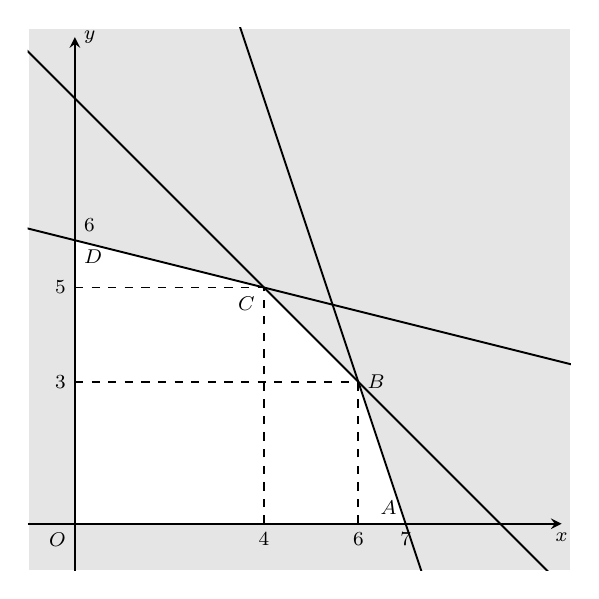
\begin{tikzpicture}[line width=1pt,>=stealth,x=1cm,y=1cm,scale=0.6,line width=0.7pt]
				\clip (-1,-1) rectangle (10.5,10.5);
				\draw[color=white,fill=black!10] (-1,-1) rectangle (10.5,10.5);
				\draw [color=white,fill=white](0,6)--(4,5)--(6,3)--(7,0)--(0,0)--cycle;
				\draw (7,0) node[above left]{\footnotesize$A$};
				\draw (7,0) node[below]{\footnotesize$7$};
				\draw (6,3) node[right]{\footnotesize$B$};
				\draw[dashed] (0,3)--(6,3);
				\draw (0,3) node[left]{\footnotesize$3$};
				\draw[dashed] (6,0)--(6,3);
				\draw (6,0) node[below]{\footnotesize$6$};
				\draw (4,5) node[below left]{\footnotesize$C$};
				\draw[dashed] (0,5)--(4,5);
				\draw (0,5) node[left]{\footnotesize$5$};
				\draw[dashed] (4,0)--(4,5);
				\draw (4,0) node[below]{\footnotesize$4$};
				\draw (0,6) node[below right]{\footnotesize$D$};
				\draw (0,6) node[above right]{\footnotesize$6$};
				\draw[->] (-1,0)--(10.3,0)
				node[below]{\footnotesize $ x $};
				\draw[->] (0,-1)--(0,10.3)
				node[right]{\footnotesize $ y $};
				\draw (0,0) node[below left]{\footnotesize $ O$};
				\draw[smooth,domain=-5:24] plot (\x,{-3*\x+21});
				\draw[smooth,domain=-5:24] plot (\x,{-\x+9});
				\draw[smooth,domain=-5:24] plot (\x,{-0.25*\x+6});
			\end{tikzpicture}
		\end{center}
		Ta có $ f(0;0)=0$; $f(7;0)=42$; $f(6;3)=60$; $f(4;5)=64$; $f(0;6)=48$.\\
		Suy ra $ f(4;5) $ là giá trị lớn nhất của hàm số $ f(x;y) $ trên miền nghiệm của hệ $ (I)$.\\
		Vậy để đạt được số điểm thưởng cao nhất, đội chơi cần pha chế $4$ cốc đồ uống loại $A$, $5$ cốc đồ uống loại $B$.\\
		Khi đó $x+y=4+5=9$.
	}
\end{ex}
%câu 8
\begin{ex}%[Dự án đề cương 3 khối NH24-25 Đợt 1-Nguyễn Tiến Liên]%[0D2V2-2]
	Một gia đình cần ít nhất $900$ đơn vị protein và $400$ đơn vị lipit trong thức ăn mỗi ngày. Mỗi ki-lô-gam thịt bò chứa $800$ đơn vị protein và $200$ đơn vị lipit. Mỗi ki-lô-gam thịt lợn (heo) chứa $600$ đơn vị protein và $400$ đơn vị lipit. Biết rằng gia đình này chỉ mua nhiều nhất là $1{,}6$ kg thịt bò và $1{,}1$ kg thịt lợn; giá $1$ kg thịt bò là $200\,000$ đồng, $1$ kg thịt lợn là $160\,000$ đồng. Gia đình đó cần mua $m$ kg thịt bò và $n$ kg thịt lợn để đảm bảo cung cấp
	đủ lượng protein, lipit cho gia đình và có chi phí là ít nhất. Tính giá trị $m+n$ với $m$; $n$ là các số hữu tỉ.
	\loigiai{
		Gọi $x$, $y$ lần lượt là số ki-lô-gam thịt bò và thịt lợn mà gia đình đó mua trong một ngày với $0\leq x \leq 1{,}6$; $0\leq y \leq 1{,}1$.\\
		Số đơn vị protein gia đình có là $800x+600y$.\\
		Số đơn vị lipit gia đình có là $200x+400y$.\\
		Theo bài ra, ta có $\heva{&0\leq x\leq 1{,}6\\	&0\leq y\leq 1{,}1\\
			&800x+600y \geq 900\\&200x+400y \geq 400} \Leftrightarrow\heva{&0\leq x\leq 1{,}6\\&0\leq y\leq 1{,}1\\&8x+6y \geq 9\\
			&x+2y \geq 2.}$\qquad $(II)$\\
		Số tiền gia đình đã dùng để mua thịt bò và thịt lợn là
		$f(x;y)=200\,000x+160\,000y$ (đồng).\\
		Ta tìm $x$, $y$ là nghiệm của hệ bất phương trình $(II)$ để $f(x;y)=200\,000x+160\,000y$ đạt giá trị nhỏ nhất.\\
		Trước hết, ta biểu diễn miền nghiệm của hệ bất phương trình $(II)$.
			\begin{center}
				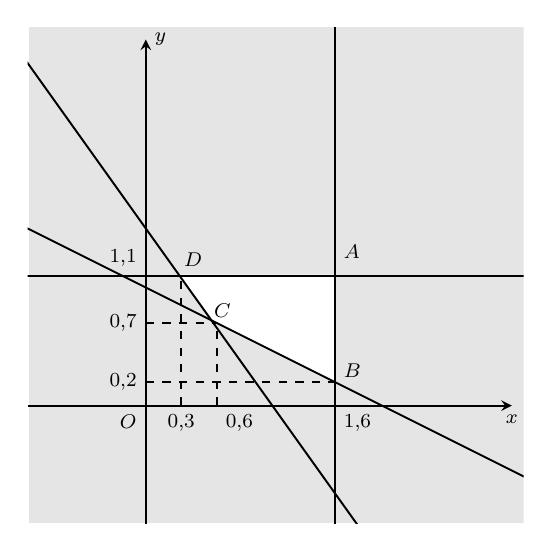
\begin{tikzpicture}[>=stealth,x=1cm,y=1cm,scale=1.5,font=\footnotesize,line width=0.7pt]
					\clip (-1,-1) rectangle (3.2,3.2);
					\draw[color=white,fill=black!10] (-1,-1) rectangle (3.3,3.3);
					\draw[color=white,fill=white] (0.3,1.1)--(1.6,1.1)--(1.6,0.2)--(0.6,0.7)--cycle;
					\draw[->] (-1,0)--(3.1,0)
					node[below]{\footnotesize $ x $};
					\draw[->] (0,-1)--(0,3.1)
					node[right]{\footnotesize $ y $};
					\draw (0,0) node[below left]{\footnotesize $ O$};
					\draw[smooth,domain=-4:4] plot (\x,{-1.4*\x+1.5});
					\draw[smooth,domain=-4:4] plot (\x,{-0.5*\x+1});
					\draw[smooth,domain=-4:4] plot (\x,{1.1});
					\draw[-] (1.6,-4) -- (1.6,4);
					\draw (1.6,1.3) node[right]{$A$};
					\draw (1.6,0.3) node[right]{ $B$};
					\draw (0.5,0.8) node[right]{ $C$};
					\draw[dashed] (0.6,0)--(0.6,0.7);
					\draw (0.6,0) node[below right]{\footnotesize$0{,}6$};
					\draw (1.6,0) node[below right]{\footnotesize$1{,}6$};
					\draw[dashed] (0,0.7)--(0.6,0.7);
					\draw (0,0.7) node[left]{\footnotesize$0{,}7$};
					\draw (0,1.1) node[above left]{\footnotesize$1{,}1$};
					\draw (0.4,1.1) node[above]{$D$};
					\draw (0.3,0) node[below]{\footnotesize$0{,}3$};
					\draw[dashed] (0.3,0)--(0.3,1.1);
					\draw (0,0.2) node[left]{\footnotesize$0{,}2$};
					\draw[dashed] (0,0.2)--(1.6,0.2);
				\end{tikzpicture}
			\end{center}
		Miền nghiệm của hệ bất phương trình $ (II) $ là tứ giác $ ABCD $ (kể cả biên).\\
		Hàm số $ f(x;y)=f(x;y)=200\,000x+160\,000y$ sẽ đạt giá trị nhỏ nhất khi $ (x ; y) $ là tọa độ của một trong các đỉnh $ A(1{,}6 ; 1{,}1) $, $ B(1{,}6 ; 0{,}2) $, $ C(0{,}6 ; 0{,}7) $, $ D(0,3 ; 1{,}1)$.\\
		Ta có $ f(1{,}6 ; 1{,}1)=496\,000$; $ f(1{,}6 ; 0{,}2)=352\,000$; $ f(0{,}6 ; 0{,}7)=232\,000$; $ f(0,3 ; 1{,}1) =236\,000$.\\
		Suy ra $ f(x;y) $ nhỏ nhất khi $ (x;y)=(0{,}6;0{,}7) $. \\
		Do đó gia đình này cần phải mua $ 0{,}6 $ kg thịt bò và $ 0{,}7 $ kg thịt lợn để số tiền bỏ ra là ít nhất. \\
		Khi đó $m+n=0{,}6+0{,}7=1{,}3$.
	}
\end{ex}
%câu 9
\begin{ex}%[Dự án đề cương 3 khối NH24-25 Đợt 1-Nguyễn Tiến Liên]%[0D2V2-2]
	Nhân dịp tết Trung thu, xí nghiệp sản xuất bánh muốn sản xuất hai loại bánh: bánh nướng và bánh dẻo. Để sản xuất hai loại bánh này, xí nghiệp cần đường, bột mì, trứng, mứt bí, lạp xưởng. Xí nghiệp đã nhập về $600$ kg bột mì và $240$ kg đường, các nguyên liệu khác luôn đáp ứng được số lượng mà xí nghiệp cần. Mỗi chiếc bánh nướng cần $120$ g bột mì, $60$ g đường. Mỗi chiếc bánh dẻo cần $160$ g bột mì và $40$ g đường. Theo khảo sát thị trường, lượng bánh dẻo tiêu thụ không vượt quá ba lần lượng bánh nướng và sản phẩm của xí nghiệp sản xuất luôn được tiêu thụ hết. Mỗi chiếc bánh nướng lãi $8\,000$ đồng, mỗi chiếc bánh dẻo lãi $6\,000$ đồng. Để đáp ứng nhu cầu thị trường; đảm bảo lượng bột mì, đường không vượt quá số lượng mà xí nghiệp đã chuẩn bị và vẫn thu được lợi nhuận cao nhất thì xí nghiệp phải sản xuất $m$ chiếc bánh nướng và $n$ chiếc bánh dẻo, với $m$, $n$ là các số tự nhiên. Tính giá trị $\dfrac{m+n}{6}$.
	\loigiai{
		Gọi $x$, $y$ (chiếc) là số lượng bánh nướng, bánh dẻo mà xí nghiệp cần sản xuất. Trong đó $0< x$, $0< y$ với $x$, $y \in \mathbb{N}^{*}$.\\
		Khối lượng bột mì cần dùng là $0{,}12x+0{,}16y$ (kg).\\
		Khối lượng đường cần dùng là $0{,}06x+0{,}04y$ (kg).\\
		Ta có $0{,}12x+0{,}16y \leq 600$ hay $3x+4y \leq 15\,000$;\\
		$0{,}06x+0{,}04y \leq 240$ hay $3x+2y \leq 12\,000$.\\
		Số tiền lãi thu được là $T=8x+6y$ (nghìn đồng). \\
		Ta  tìm $x$, $y$ là nghiệm của hệ bất phương trình $\heva{&3x+4y \leq 15\,000\\&3x+2y \leq 12\,000\\&y\leq 3x \\&x\geq 0\\	&y\geq 0}$ \qquad$(III)$ để $T=8x+6y$ đạt giá trị lớn nhất.\\
		Trước hết, ta biểu diễn miền nghiệm của hệ bất phương trình $(III)$.
		\begin{center}
			\begin{center}
				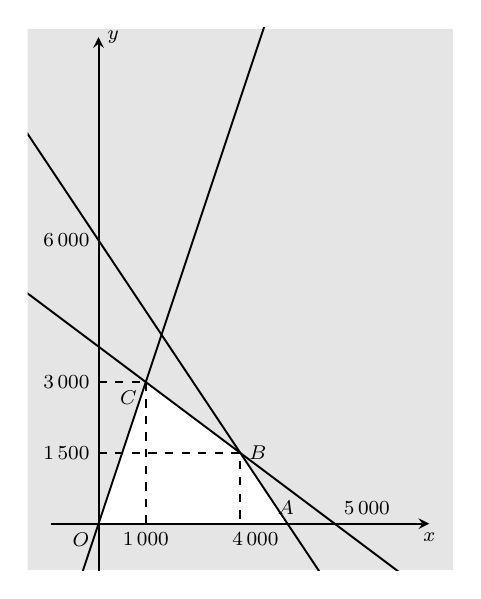
\begin{tikzpicture}[line width=1pt,>=stealth,x=1cm,y=1cm,scale=0.6,line width=0.7pt]
					\clip (-1.5,-1) rectangle (7.5,10.5);
					\draw[color=white,fill=black!10] (-2,-1) rectangle (10.5,10.5);
					\draw [color=white,fill=white](0,0)--(1,3)--(3,1.5)--(4,0)--cycle;
					\draw (3.6,0) node[above right]{\footnotesize$A$};
					\draw (4,0) node[below left]{\footnotesize$4\,000$};
					\draw (3,1.5) node[right]{\footnotesize$B$};
					\draw[dashed] (0,3)--(1,3);
					\draw (0,3) node[left]{\footnotesize$3\,000$};
					\draw[dashed] (1,0)--(1,3);
					\draw (1,3) node[below left]{\footnotesize$C$};
					\draw (0,6) node[left]{\footnotesize$6\,000$};
					\draw (1,0) node[below]{\footnotesize$1\,000$};
					\draw (5,0) node[above right]{\footnotesize$5\,000$};
					\draw[dashed] (0,1.5) node[left]{\footnotesize$1\,500$}--(3,1.5)--(3,0);
					\draw[->] (-1,0)--(7,0)
					node[below]{\footnotesize $x$};
					\draw[->] (0,-1)--(0,10.3)
					node[right]{\footnotesize $y$};
					\draw (0,0) node[below left]{\footnotesize $O$};
					\draw[smooth,domain=-5:24] plot (\x,{3*\x});
					\draw[smooth,domain=-5:24] plot (\x,{-1.5*\x+6});
					\draw[smooth,domain=-5:24] plot (\x,{-3/4*\x+15/4});
				\end{tikzpicture}
			\end{center}
		\end{center}
		Miền nghiệm của hệ bất phương trình là miền tứ giác $OABC$ với $O(0; 0)$, $A(4\,000;0)$, $B(3\,000; 1\,500)$, $C(1\,000;3\,000)$.\\
		%Hình vẽ
		Lập bảng giá trị của $T$ ta được
		\begin{center}
			\renewcommand{\arraystretch}{1.3}
			\begin{tabular}{|>{\centering\arraybackslash}m{3cm}|
					>{\centering\arraybackslash}m{3cm}|
					>{\centering\arraybackslash}m{3cm}|
					>{\centering\arraybackslash}m{3cm}|
					>{\centering\arraybackslash}m{3cm}|
				}
				\hline
				Đỉnh & $O(0;0)$ & $A(4\,000;0)$ & $B(3\,000; 1\,500)$& $C(1\,000;3\,000)$ \\
				\hline
				$T$ & $0$ & $32\,000$ & $33\,000$&$26\,000$ \\
				\hline
			\end{tabular}
		\end{center}
		Từ bảng trên suy ra $T$ đạt giá trị lớn nhất bằng $33\,000$ nghìn đồng hay $33$ triệu đồng tại $x=3\,000$; $y=1\,500$.\\
		Vậy để đạt được tiền lãi cao nhất, xí nghiệp nên sản xuất $3\,000$ chiếc bánh nướng và $1\,500$ chiếc bánh dẻo.\\
		Khi đó $\dfrac{m+n}{6}=\dfrac{3\,000+1\,500}{6}=750$.
	}
\end{ex}
%câu 10
\begin{ex}%[Dự án đề cương 3 khối NH24-25 Đợt 1-Nguyễn Tiến Liên]%[0D2V2-2]
	Một xưởng sản xuất hai loại sản phẩm là sản phẩm loại $I$ và sản phẩm loại $II$:
	Mỗi kg sản phẩm loại $I$ cần $2$ kg nguyên liệu và $30$ giờ, thu lời được $40$ nghìn.\\
	Mỗi kg sản phẩm loại $II$ cần $4$ kg nguyên liệu và $15$ giờ, thu lời được $30$ nghìn.\\
	Xưởng có $200$ kg nguyên liệu và $1\,200$ giờ làm việc tối đa. Để có mức lời cao nhất xưởng sẽ sản xuất $m$ sản phẩm loại $I$ và $n$ sản phẩm loại $II$, với $m$, $n$ là các số tự nhiên. Tính giá trị $m+2n$.
	\loigiai{
		Gọi $x$, $y$ lần lượt là số kg sản phẩm loại $I$ và loại $II$ mà xưởng sản xuất được.\\
		Tổng nguyên liệu được dùng là $2x+4y$ (kg); tổng thời gian sản xuất là $30x+15y$ (giờ); $x$, $y \geq 0$.\\
		Ta có hệ bất phương trình $\heva{&2x+4y \leq 200\\
			&30x+15y \leq 1\,200\\&x\geq 0\\&y\geq 0} \Leftrightarrow\heva{&x+2y \leq 100\\&2x+y \leq 80\\&x\geq 0\\	&y\geq 0.}$\\
		Vẽ trên cùng hệ trục các đường thẳng $d_1\colon x+2y=100$, $d_2\colon 2x+y=80$, $d_3\colon y=0$, $d_4\colon x=0$.\\
		Ta có điểm $M(1; 1)$ thuộc miền nghiệm của hệ bất phương trình vì khi thay tọa độ điểm này vào hệ $\heva{&1+2\cdot 1\leq 100\\	&2\cdot 1+1\leq 80\\
			&1\geq 0\\	&1\geq 0}$ (đúng).
		\begin{center}
			\begin{tikzpicture}[thick, line cap=round, line join=round, font=\footnotesize,scale=.6]
				\def\xmin{-1}
				\def\xmax{12}
				\def\ymin{-1}
				\def\ymax{9}
				\clip (\xmin,\ymin) rectangle (\xmax,\ymax);
				\fill[pattern=north east lines,pattern color=black,opacity=0.45] (\xmin,\ymin)--(\xmax,\ymin)--(\xmax,\ymax)--(\xmin,\ymax)--cycle;
				\fill[color=white] (0,0)--(0,5)--(2,4)--(4,0)--cycle;
				\draw[-stealth] (\xmin,0)--(\xmax,0)node[above left]{$x$};
				\draw[-stealth] (0,\ymin)--(0,\ymax)node[below right]{$y$};
				\draw[domain=\xmin:\xmax] plot(\x,{8-2*(\x)});
				\draw[domain=\xmin:\xmax] plot(\x,{5-0.5*(\x)});
				\node[below left] at (0,0) {$O$};
				\node[below left] at (0,5) {$A$};
				\node[above right] at (2,4) {$B$};
				\node[below left] at (4,0) {$C$};
				\draw[dashed](2,0)--(2,4)--(0,4);
				\draw (2,0) node[below]{$20$};
				\draw (0,4) node[left]{$40$};
			\end{tikzpicture}
		\end{center}
		Gạch bỏ các phần không thuộc miền nghiệm của mỗi bất phương trình trong hệ (nửa mặt phẳng có bờ là các đường thẳng $d_1$, $d_2$, $d_3$, $d_4$ và không chứa điểm $M$). Khi đó miền nghiệm của hệ bất phương trình chính là miền của tứ giác $OABC$ (kể cả các cạnh của tứ giác đó) với $O(0; 0)$, $A(0;50)$, $B(20;40)$, $C(40; 0)$.\\
		Lãi thu về từ việc sản xuất hai sản phẩm là $F(x; y)=40x+30y$ (nghìn đồng).\\
		Tại $O(0; 0)$, ta có $F(0; 0)=0$;\\
		Tại $A(0; 50)$, ta có $F(0; 50)=1\,500$;\\
		Tại $B(20; 40)$, ta có $F(20; 40)=2\,000$;\\
		Tại $C(40; 0)$, ta có $F(40; 0)=1\,600$.\\
		Vậy lãi suất cao nhất thu được bằng $2\,000\,000$ đồng, khi đó $x=20$, $y=40$ (tức là xưởng cần sản xuất ra $20$ sản phẩm loại $I$ và $40$ sản phẩm loại $II$).\\
		Khi đó $\heva{&m=20\\&n=40} \Rightarrow m+2n=20+2\cdot 40=100$.}
\end{ex}
%câu 11
\begin{ex}%[Dự án đề cương 3 khối NH24-25 Đợt 1-Nguyễn Tiến Liên]%[0D2V2-3]
	Một hộ nông dân định trồng dứa và củ đậu trên diện tích $8$ ha. Trên diện tích mỗi ha, nếu trồng dứa thì cần $20$ công và thu $3$ triệu đồng, nếu trồng củ đậu thì cần $30$ công và thu $4$ triệu đồng. Để thu được nhiều tiền nhất hộ nông dân cần trồng $m$ ha dứa và $n$ ha củ đậu, biết rằng $m$, $n$ là các số tự nhiên và tổng số công không quá $180$. Tính giá trị $m+2n$
	\loigiai{
		\immini{Gọi $x$, $y$  lần lượt là số ha trồng dứa và củ đậu. Điều kiện $0\leq x\leq 8$ và $0\leq y\leq 8$.\\
			Tổng diện tích trồng là  $x+y$ (ha), tổng số công cần thiết là  $20x+30y$ (công). \\
			Số tiền thu được là  $T(x;y)=3x+4y$ (triệu đồng).\\
			Ta có hệ bất phương trình $$\heva{&0\leq x\leq 8\\&0\leq y\leq 8\\&x+y\le 8\\&20x+30y\leq 180}\Leftrightarrow\heva{&0\leq x\leq 8\\&0\leq y\leq 8\\&x+y\le 8\\&2x+3y\leq 18.}$$
			Miền nghiệm của hệ trên là miền tứ giác $OABC$ (kể cả biên) với các đỉnh $O(0;0)$; $A(0;6)$; $B(6;2)$; $C(8;0)$.
		}{\begin{tikzpicture}[line join=round, line cap=round,>=stealth,thick,scale=0.6]
				\tikzset{label style/.style={font=\footnotesize}}
				\begin{scope}
					\clip (-1,-1) rectangle (10,10);
					\fill[pattern=north east lines,opacity=0.45] (-3,11)--(11,11)--(11,-3)--cycle;
					\fill[pattern=north east lines,opacity=0.45] (-7,10.67)--(11,10.67)--(11,-1.33)--cycle;
					\fill[pattern=north east lines,opacity=0.45] (0,-1)--(-1,-1)--(-1,10)--(0,10)--cycle;
					\fill[pattern=north east lines,opacity=0.45] (-1,0)--(-1,-1)--(10,-1)--(10,0)--cycle;
					\draw (-2,10)--(9,-1) node [pos=0.45, above, sloped] {$x+y-8=0$};
					\draw (-6,10)--(10.5,-1) node [pos=0.55, below, sloped] {$2x + 3y -18=0$};
				\end{scope}
				\draw[->] (-1,0)--(10,0) node[below]{$x$};
				\draw[->] (0,-1)--(0,10) node[left]{$y$};
				\draw (0,0) node[below left]{$O$} (0,8)node[right]{$8$} (0,6)node[left]{$6$} (0,6+0.1)node[right]{$A$} (8,0)node[below]{$8$} (9,0)node[below]{$9$} (6,2)node[above]{$B$} (8,0)node[above]{$C$};
				\draw[dashed](6,0)node[below]{$6$}--(6,2)--(0,2)node[left]{$2$};
		\end{tikzpicture}}
		\noindent	Khi đó $T(x;y)$ đạt giá trị lớn nhất tại một trong các đỉnh trên. Ta có
		\begin{multicols}{2}
			\begin{itemize}
				\item $T(0;0)=0$.
				\item $T(0;6)=24$.
				\item $T(6;2)=26$.
				\item $T(8;0)=24$.
			\end{itemize}
		\end{multicols}
		\noindent	Vậy giá trị lớn nhất của $T( x;y)$ bằng $26$ (triệu đồng), khi đó $x=6$, $y=2$ (tức là hộ nông dân cần trồng $6$ ha dứa và $2$ ha củ đậu để có thể thu lại số tiền nhiều nhất).\\
		Khi đó $m=6$ và $n=2$ nên $m+2n=10$.
	}
\end{ex}
%câu 12
\begin{ex}%[Dự án đề cương 3 khối NH24-25 Đợt 1-Nguyễn Tiến Liên]%[0D2V2-3]
	Có ba nhóm máy X, Y, Z dùng để sản xuất ra hai loại sản phẩm I và II. Để sản xuất một đơn vị sản phẩm mỗi loại lần lượt phải dùng các máy thuộc các nhóm khác nhau. Số máy trong một nhóm và số máy của từng nhóm cần thiết để sản xuất ra một đơn vị sản phẩm thuộc mỗi loại được dùng cho trong bảng sau
	\begin{center}
		\begin{tikzpicture}[>=stealth,line join=round,line cap=round,scale=1]
			\draw (0.25,-.5)node{Nhóm} (4,-.25)node{Số máy trong nhóm} (10,0.1)node{Số máy trong từng nhóm } (4,-.75)node{nguyên liệu đang có} (10,-0.4)node{để sản xuất ra một đơn vị}
			(8,-1.25)node{Loại I} (12,-1.25)node{Loại II}
			(0.25,-2)node{X} (0.25,-3)node{Y} (0.25,-4)node{Z}
			(4,-2)node{$10$} (4,-3)node{$4$} (4,-4)node{$12$}
			(8,-2)node{$2$} (8,-3)node{$0$} (8,-4)node{$2$}
			(12,-2)node{$2$} (12,-3)node{$2$} (12,-4)node{$4$};
			\draw (-1.5,.5)--(14,0.5)--(14,-4.5)--(-1.5,-4.5)--cycle (2,0.5)--(2,-4.5) (6,.5)--(6,-4.5) (10,-.75)--(10,-4.5) (-1.5,-1.5)--(14,-1.5) (6,-.75)--(14,-.75) (-1.5,-2.5)--(14,-2.5) (-1.5,-3.5)--(14,-3.5);
		\end{tikzpicture}
	\end{center}
	Một đơn vị sản phẩm loại I lãi $3$ nghìn đồng, một đơn vị sản phẩm loại II lãi $5$ nghìn đồng. Để cho tổng số tiền lãi thu được là cao nhất thì đơn vị phải sản xuất $m$ sản phẩm loại I và $n$ sản phẩm loại II, với $m$, $n$ là các số tự nhiên. Tính giá trị $m-n$.
	\loigiai{
		Gọi $x$ là số đơn vị sản phẩm loại I, $y$ là số đơn vị sản phẩm loại II sản xuất ra. \\
		Như vậy tiền lãi có được là $F(x;y)=3x+5y$ (nghìn đồng).\\
		Theo giả thiết:\\
		Số máy cần dùng nhóm X là $2x+2y$ (máy); \\
		Số máy cần dùng ở nhóm Y là $0x+2y$ (máy); \\
		Số máy cần dùng ở nhóm Z là $2x+4y$ (máy).\\
		Ta có hệ bất phương trình $\heva{&2x+2y\le 10\\&2y\le 4\\&2x+4y\le 12\\&x\ge 0\\&y\ge 0.}$ hay $\heva{&x+y\le 5\\&y\le 2\\&x+2y\le 6\\&x\ge 0\\&y\ge 0.}$
		\begin{center}
			\begin{tikzpicture}[line join=round, line cap=round,>=stealth,thick]
				\tikzset{label style/.style={font=\footnotesize}}
				\begin{scope}
					\clip (-1,-1) rectangle (8,6);
					\fill[pattern=north east lines,opacity=0.45] (-2,7)--(9,7)--(9,-4)--cycle;
					\fill[pattern=north east lines,opacity=0.45] (-1,2)--(-1,6)--(8,6)--(8,2)--cycle;
					\fill[pattern=north east lines,opacity=0.45] (-7,6.5)--(9,6.5)--(9,-1.5)--cycle;
					\fill[pattern=north east lines,opacity=0.45] (0,-1)--(-1,-1)--(-1,6)--(0,6)--cycle;
					\fill[pattern=north east lines,opacity=0.45] (-1,0)--(-1,-1)--(8,-1)--(8,0)--cycle;
					\draw (-1,6)--(6,-1) node [pos=0.45, above, sloped]{$x+y=5$};
					\draw (-1,2)--(8,2) node [pos=0.7, above, sloped] {$y=2$};
					\draw (-6,6)--(8,-1) node [pos=0.5, above, sloped]{$x+2y=6$};
				\end{scope}
				\draw[->] (-1,0)--(8,0) node[below]{$x$};
				\draw[->] (0,-1)--(0,6) node[left]{$y$};
				\draw (0,0) node[below left]{$O$} (0,2)node[below left]{$2$} (0,2)node[below right]{$A$} (2,2)node[below]{$B$} (4,1)node[below]{$C$} (5,0)node[above]{$D$} (5,0)node[below]{$5$};
			\end{tikzpicture}
		\end{center}
		Miền nghiệm của hệ trên được biểu diễn là miền của ngũ giác $OABCD$ với $O(0;0)$, $A( 0;2)$, $B( 2;2)$, $C(4;1)$, $D(5;0)$.\\
		Xét $O(0;0)$, ta có $F(0;0)=3\cdot0+5\cdot0=0$;\\
		Xét $A(0;2)$, ta có $F(0;2)=3\cdot0+5\cdot2=10$;\\
		Xét $B(2;2)$, ta có $F(2;2)=3\cdot2+5\cdot2=16$;\\
		Xét $C(4;1)$, ta có $F(4;1)=3\cdot4+5\cdot1=17$;\\
		Xét $D(5;0)$, ta có $F(5;0)=3\cdot5+5\cdot0=15$.\\
		Từ các kết quả trên, ta thấy khoản lãi lớn nhất ($F(x;y)$ lớn nhất) bằng $17$ (ngàn đồng), khi đó người ta cần làm ra $4$ sản phẩm loại I và $1$ sản phẩm loại II (tức là $x=4$, $y=1$).\\
		Do vậy $m=4$ và $n=1$ nên $m-n=3$.
	}
\end{ex}
%câu 13
\begin{ex}%[Dự án đề cương 3 khối NH24-25 Đợt 1-Nguyễn Tiến Liên]%[0D2V2-3]
	Bác Năm dự định trồng ngô và đậu xanh trên một mảnh đất có diện tích $8$ hecta (ha). Nếu trồng $1$ ha ngô thì cần $20$ ngày công và thu được $40$ triệu đồng. Nếu trồng $1$ ha đậu xanh thì cần $30$ ngày công và thu được $50$ triệu đồng. Để thu được nhiều tiền nhất thì bác Năm cần trồng $m$ ha ngô và $n$ ha đậu xanh, với $m$, $n$ là các số tự nhiên. Tính giá trị $m+n$. Biết rằng, bác Năm chỉ có thể sử dụng không quá $180$ ngày công cho việc trồng ngô và đậu xanh.
	\loigiai{
		Gọi $x$ là số hecta đất trồng ngô và $y$ là số hecta đất trồng đậu xanh. Điều kiện $0\leq x\leq 8$ và $0\leq y\leq 8$.
		\begin{itemize}
			\item Diện tích canh tác không vượt quá $8$ ha nên $x+y \leq 8$.
			\item Số ngày công sử dụng không vượt quá $180$ nên $20x+30y \leq 180$.
		\end{itemize}
		Từ đó, ta có hệ bất phương trình
		$\heva{&x+y \leq 8 \\& 20x+30y \leq 180 \\& 0\leq x\leq 8 \\& 0\leq y\leq 8.}$\\
		Biểu diễn miền nghiệm của hệ bất phương trình này trên hệ truc toạ độ $Oxy$, ta được miền tứ giác $OABC$.\\
		Tọa độ các đỉnh của tứ giác đó là $O(0;0)$, $A(0;6)$, $B(6;2)$, $C(8;0)$.\\
		Gọi $F$ là số tiền (đơn vị: triệu đồng) bác Năm thu được, ta có $F=40x+50y$.\\
		Ta phải tìm $x$, $y$ thỏa mãn hệ bất phương trình sao cho $F$ đạt giá trị lớn nhất, nghĩa là tìm giá trị lớn nhất của biểu thức $F=40x+50y$ trên miền tứ giác $OABC$.
		\begin{center}
			\begin{tikzpicture}[line join=round, line cap=round,>=stealth,thick,scale=0.8]
				\tikzset{label style/.style={font=\footnotesize}}
				\begin{scope}
					\clip (-1,-1) rectangle (10,10);
					\fill[pattern=north east lines,opacity=0.45] (-3,11)--(11,11)--(11,-3)--cycle;
					\fill[pattern=north east lines,opacity=0.45] (-7,10.67)--(11,10.67)--(11,-1.33)--cycle;
					\fill[pattern=north east lines,opacity=0.45] (0,-1)--(-1,-1)--(-1,10)--(0,10)--cycle;
					\fill[pattern=north east lines,opacity=0.45] (-1,0)--(-1,-1)--(10,-1)--(10,0)--cycle;
					\draw (-2,10)--(9,-1) node [pos=0.45, above, sloped] {$x+y-8=0$};
					\draw (-6,10)--(10.5,-1) node [pos=0.55, below, sloped] {$20x + 30y -180=0$};
				\end{scope}
				\draw[->] (-1,0)--(10,0) node[below]{$x$};
				\draw[->] (0,-1)--(0,10) node[left]{$y$};
				\draw (0,0) node[below left]{$O$} (0,8)node[right]{$8$} (0,6)node[left]{$6$} (0,6+0.1)node[right]{$A$} (8,0)node[below]{$8$} (9,0)node[below]{$9$} (6,2)node[above]{$B$} (8,0)node[above]{$C$};
				\draw[dashed](6,0)node[below]{$6$}--(6,2)--(0,2)node[left]{$2$};
			\end{tikzpicture}
		\end{center}
		Tính các giá trị của biểu thức $F$ tại các đỉnh của đa giác, ta có\\
		Tại $O(0;0)\colon F=40\cdot 0+50\cdot 0=0$.\\
		Tại $A(0;6)\colon F=40\cdot 0+50\cdot 6=300$.\\
		Tại $B(6;2)\colon F=40\cdot 6+50\cdot 2=340$.\\
		Tại $C(8;0)\colon F=40\cdot 8+50\cdot 0=320$.\\
		$F$ đạt giá trị lớn nhất bằng $340$ tại $B(6;2)$.\\
		Vậy để thu được nhiều tiền nhất, bác Năm cần trồng $6$ ha ngô và $2$ ha đậu xanh.\\
		Khi đó $m=6$ và $n=2$ thì $m+n=8$.
	}
\end{ex}